\documentclass[a4paper]{article}

%Russian-specific packages
%--------------------------------------
\usepackage[T2A]{fontenc}
\usepackage[utf8]{inputenc}
\usepackage[english, russian]{babel}
%for search in russian
\usepackage{cmap}
%--------------------------------------

%Math-specific packages
%--------------------------------------
\usepackage{amsmath}
\usepackage{amssymb}

%Format-specific packages
%--------------------------------------
\usepackage[left=1cm,
            right=1cm,
            top=1cm,
            bottom=1cm,
            bindingoffset=0cm]{geometry}
%--------------------------------------

% for theorems, lemmas and definitions
%--------------------------------------
\usepackage{amsthm}

\counterwithin*{equation}{section}

\newtheorem{theorem}{Теорема}[section]
\newtheorem {lemma}{Лемма}[section]
\newtheorem*{statement}{Утверждение}
\newtheorem*{lemma*}{Лемма}
\newtheorem*{proposition}{Предложение}

\theoremstyle{definition}
\newtheorem {definition}{Опр.}[section]
\newtheorem {example}{Пример}[section]
\newtheorem*{example*}{Пример}
\newtheorem {task}{Задача}[section]
\newtheorem*{task*}{Задача}

\theoremstyle{remark}
\newtheorem {remark}{Замечание}[section]
\newtheorem*{remark*}{Замечание}
\newtheorem {corollary}{Следствие}[section]
\newtheorem*{corollary*}{Следствие}

%--------------------------------------

% For graphics
%--------------------------------------
\usepackage{tikz}
\usetikzlibrary{
  % for faster compilation
  external
  % for cool arrows
  , arrows.meta
  % for angles
  , angles
  , quotes
  , babel
}
\tikzexternalize

%--------------------------------------

% For hyperlinks
%--------------------------------------
\usepackage{float}
\usepackage[hidelinks]{hyperref}
%--------------------------------------

% My commands
%--------------------------------------
\newcommand\defin[1]{\textbf{#1}}

\newcommand*{\defeq}{\stackrel{\text{def}}{=}}

\DeclareMathOperator{\sgn}{sgn}

\def\const{ \mathrm{const} }
\def\eps{ \varepsilon }
\def\Eps{ \mathcal{E} }

\def\R{ \mathbb{R} }
\def\Z{ \mathbb{Z} }
\def\C{ \mathbb{C} }
\def\E{ \mathrm{E} }
\def\D{ \mathrm{D} }
\def\P{ \mathrm{P} }

\def\littleO{ \overline{\overline{o}} }
\def\bigO{ \underline{\underline{\mathcal{O}}} }

\newcommand*{\norm}[1]{\left\lVert#1\right\rVert}
\newcommand*{\abs}[1]{\left\lvert#1\right\rvert}

% suppress page count
\pagestyle{empty}

\includeonly{
  01/01,
  02/02,
  03/03,
  04/04,
  05/05,
  06/06,
  07/07,
  08/08,
  09/09,
  10/10,
  11/11,
  12/12,
  13/13,
  14/14,
  15/15,
  16/16,
  17/17,
  18/18,
  19/19,
  20/20,
  21/21,
  22/22,
  23/23,
  24/24,
  25/25,
  26/26,
  27/27,
  28/28,
  29/29,
  30/30,
  31/31,
  32/32,
  33/33,
  34/34,
  35/35,
  36/36,
  37/37,
  38/38,
  39/39,
  40/40,
  41/41,
  42/42,
  43/43,
  44/44,
  45/45,
  46/46,
  47/47,
  48/48,
  49/49,
  50/50,
  51/51,
  52/52,
  53/53,
  54/54,
  55/55,
  56/56,
  57/57,
  58/58,
  59/59,
  60/60,
  61/61,
  62/62,
  63/63,
  64/64,
  65/65,
  66/66,
  67/67,
  68/68,
}

\begin{document}

\section{Вычислительная погрешность. Устойчивость задачи и численного алгоритма.}

Определим вычислительную погрешность и машинную точность.
Для этого нам понадобятся основы машинной арифметики.

Наиболее распространенная форма представления действительных чисел в
компьютерах - числа с плавающей точкой. Множество $F$ чисел с плавающей
точкой характеризуется четырьмя параметрами: основанием системы
счисления $p$, разрядностью $t$ и интервалом показателей $[L;U]$. Каждое
число $x$, принадлежащее $F$, представимо в виде

\[x=\pm\left(\frac{d_1}{p}+\frac{d_2}{p^2}+\ldots+\frac{d_t}{p^t}\right)p^{\alpha};\ 0\leq d_i\leq p-1;\ i=1,\ldots,t;L\leq\alpha\leq U\]

$d_i$ называют \textit{разрядами}, $t$ - \textit{длиной мантиссы}, $\alpha$ - \textit{порядком числа}.
\textit{Мантиссой} (дробной частью) $x$ называют число в скобках.
Множество $F$ называют \textit{нормализованным} если $\forall\ x\neq0\Rightarrow d_1\neq0$.

\begin{example}
  $p=10,\ t=6$
  \[x = 1723,4835=+\left(\frac{1}{10}+\frac{7}{10^2}+\frac{2}{10^3}+\frac{3}{10^4}+\frac{4}{10^5}+\frac{8}{10^6}\right)10^4=0,172348\cdot10^4\]
\end{example}

Округление чисел при работе на компьютере с точностью $\varepsilon$ это
некоторое отображение $float:\R \rightarrow F$ удовлетворяющее условию:
\[\forall\ y\in\R,\ float(y)\in F,\ float(y)\neq0\rightarrow float(y)=y\cdot(1+\eta),|\eta|<\varepsilon\]

Таким образом относительная погрешность
\[\left|\frac{float(y)-y}{float(y)}\right|=\left|\frac{y\cdot(1+\eta)-y}{y}\right|=\left|\eta\right|\leq\varepsilon\equiv\const\]

Величина $\varepsilon$ имеет порядок $p^{1-t}$. Величину $\varepsilon$ часто называют \textit{машинной точностью}.

В современных компьютерах число с \textit{плавающей точкой}
`double' занимает 8 байт: 1 бит под знак, 11 битов под экспоненту,
оставшиеся 52 под мантиссу. Диапазон значений: $2^{\pm2^{10}}\simeq10^{\pm308}$,
машинная точность: $2^{-53}\simeq10^{-16}$.

Aлгоритмы, традиционно применяемые в точной арифметике,
могут некорректно работать при расчетах из-за конечной точности
на ЭВМ. Как следствие, к методам и постановкам задач вычислительной
математики предъявляют дополнительные требования.

\begin{enumerate}
  \item Решаемая численно задача должна быть устойчива, т.е. малое
        изменение входных параметров не должно значительно менять результат;
        \begin{example}[Неустойчивая задача]
          Рассотрим возмущенную матрицу Уилкинсона
          \[
            A(\varepsilon)=\left(\begin{array}{cccccc}
                20          & 20 &    &        &  & 0  \\
                            & 19 & 20 &        &  &    \\
                            &    & 18 & \ddots &  &    \\
                            &    &    & \ddots &  &    \\
                0           &    &    &        &  & 20 \\
                \varepsilon & 0  &    &        &  & 1
              \end{array}\right)
          \]
          Определитель этой матрицы (считаем по столбцам) равен
          \[\det(A(\varepsilon))=20!-\varepsilon\cdot20^{19}\]
          Характеристический многочлен матрицы
          \[\det(A(\varepsilon)-\lambda I)=(20-\lambda)\cdots(1-\lambda) - 20^{19}\varepsilon\]
          При $\varepsilon=0$ $\det(A(0))=20!$, а минимальное собственное число $\lambda_{min}=1$.
          Рассмотрим $\varepsilon=20^{-19}\cdot20!\approx5\cdot10^{-7}$:
          \[\det(A(5\cdot10^{-7}))\approx0\]
          То есть при достаточно малом $\varepsilon$ определитель
          матрицы изменился на $20!$, а величина наименьшего собственного значения стала равна $0$.

          Таким образом вычисление определителя является неустойчивой задачей,
          так как \textit{незначительная погрешность во входных данных может
            существенно исказить ответ}.
        \end{example}
  \item Выбранный алгоритм должен быть численно устойчив, т.е.
        ошибки округления в промежуточных вычислениях не должны искажать
        окончательный ответ;
        \begin{example}[Численно неустойчивый алгоритм]
          Вычисляется сумма $\sum_{i=1}^{10^3}1/i^2$. Какой алгоритм даст большую точность?
          \[S_0=0;\ S_n=S_{n-1}+\frac{1}{n^2},\ n=1,\ldots,10^3\]
          или
          \[R_{10^3+1}=0;\ R_{n-1}=R_n+\frac{1}{n^2},\ n=10^3,\ldots,1\]

          Рассмотрим более простой пример: в компьютерной арифметике
          надо сложить два числа при $t=5,p=10$:
          \[float(100,01) + float(0,0001)=0,10001\cdot10^3 +0,10000\cdot10^{-3}=float(100,0101)=0,10001\cdot10^3\]
          То есть сложение чисел разного порядка может привести к потере точности.

          Возвращаясь к задаче: следует воспользоваться вторым
          способом. При вычислении первым способом происходит
          потеря точности в результате сложения чисел $S_{n-1}$ и $1/n^2$,
          существенно отличающихся по величине.
        \end{example}
  \item Имеющиеся вычислительные ресурсы (память, быстродействие,
        программное обеспечение) должны позволить реализовать алгоритм и получить ответ за требуемое время.
        \begin{example}[Непозволительно долгий алгоритм]
          Метод Крамера решения систем линейных алгебраических уравнений с невырожденной матрицей
          $n \times n$ позволяет найти точное решение, вычислив $(n + 1)$ определитель матриц размерности $n \times n$.
          Оценим $T(n)$ - время работы алгоритма.

          Вычисление одного определителя методом миноров реализуется за $\sim nn!$
          арифметических действий, для вычисления $(n + 1)$ определителя потребуется
          $N \sim n(n + 1)!$ арифметических действий. Например, для $n = 20, 100$ имеем:
          \[20!\approx2.4\cdot10^{18},\ N(20)\approx10^{21};100!\approx10^{158},\ N(100)\approx10^{162}\]
          На современных компьютерах для выполнения $N(20)$ операций потребуется $3\cdot10^{139}$ лет.
        \end{example}
\end{enumerate}

\section{Линейные разностные уравнения n-го порядка.
  Теоремы о представлении общего решения однородного уравнения
  и общего решения неоднородного уравнения.
 }

\begin{definition}
  Пусть неизвестная функция $y$, заданные функции $a$, $f$
  -- функции одного целочисленного аргумента $k$.
  \[ a_0(k)y(k)+a_1(k+1)+\ldots+a_{n-1}(k)y(k+n-1)+a_n(k)y(k+n)=f(k) \Leftrightarrow Ly=f \]
  Тогда уравнение при $f(k),\ a_0(k),\ a_n(k) \neq 0$ называется
  неоднородным линейным разностным уравнением $n$-го порядка.
  Порядок -- количество начальных условий, при которых уравнение
  является разрешимым. Уравнение $Ly = 0$ называется однородным.
\end{definition}
\begin{example}
  \[S(n)=\sum_{i=0}^{n}(1+i+i^3)\underset{\text{переход к разностному уравнению}}{\Rightarrow}S_{n+1}=S_n+1+(n+1)+(n+1)^3\]
  Получили уравнение первого порядка, а в качестве начальных условий возьмем $S_0=+1+(0+1)+(0+1)^3=3$.
\end{example}
\begin{theorem}
  Пусть $y^{(1)}(k),\ldots,y^{(n)}(k)$ - произвольные линейно независимые
  решения линейного однородного разностного уравнения $n$-го порядка
  $Ly=0$, тогда общее решение можно представить в виде
  \[y(k)=\sum_{i=1}^{n}c_iy^{(i)}(k)\]
  $c_i$ в данной записи порождаются из начальных условий задачи.
\end{theorem}
\begin{proof}
  \begin{enumerate}
    \item Покажем, что если функция совпадает на $n$ точках,
          то она совпадает и на всех остальных.

          Так как наше уравнение имеет порядок $n$, то
          $\exists$ ${a_0(k)},\ldots,a_{n-1}(k)\neq0$.

          Перепишем исходное уравнение в двух видах
          \begin{equation}\label{eq:lin:forward}
            y(k+n)=-\sum_{i=0}^{n-1}\frac{a_i(k)}{a_n(k)}y(k+i)
          \end{equation}
          \begin{equation}\label{eq:lin:backward}
            y(k)=-\sum_{i=1}^{n}\frac{a_i(k)}{a_0(k)}y(k+i)
          \end{equation}

          Таким образом, если мы знаем $n$ точек $y(k_0),\ldots,y(k_0+n-1)$,
          то из равенства~\eqref{eq:lin:forward} мы можем восстановить $y(k)\ \forall\ k\geq k_0+n$,
          а из равенства~\eqref{eq:lin:backward} мы можем восстановить $y(k)\ \forall\ k\leq k_0$.
          То есть если мы имеем $n$ точек, то мы можем однозначно восстановить
          все решение, а это значит, что если два решения совпадают на
          $n$ точках, то они тождественно равны $\forall\ k$.
    \item Дано $\left\{y^{(i)}(k)\right\}_{i=1}^{n}$ -- $n$
          линейно независимых решений нашего уравнения. Зафиксировав
          $k=k_0,\ldots,k_{n-1}$ мы получим базис в пространстве $\R^n$.
          В этом базисе мы можем выразить искомое решение как линейную
          комбинацию элементов базиса
          \[y(k)=\sum_{i=1}^{n}c_iy^{(i)}(k),\ k=k_0,\ldots,k_{n-1}\]
          Из предыдущего пункта знаем, что если решение совпадает на $n$
          точках, то совпадает и везде, то есть
          \[y(k)=\sum_{i=1}^{n}c_iy^{(i)}(k),\ \forall k\]
  \end{enumerate}
\end{proof}

\begin{definition}
  \textit{Общим} решением задачи называют то решение, которое
  можно получить из любых начальных условий.
\end{definition}

\begin{theorem}
  Пусть $y^o(k)$ - общее решение однородной задачи $Ly=0$.
  Пусть $y^1(k)$ - некоторое частное решение неоднородной
  задачи $Ly=f$. Тогда любое решение неоднородной задачи
  можно представить в виде
  \[y(k)=y^o(k)+y^1(k)\]
\end{theorem}
\begin{proof}
  Пусть $y(k)$ -- какое-либо решение задачи $Ly=f$,
  $y^1(k)$ -- некоторое частное решение этой же задачи. Тогда
  $y(k)-y^1(k)$ является решением задачи $Ly=0$:
  \[L(y(k)-y^1(k))=L(y(k))-L(y^1(k))=f(k)-f(k)=0\Rightarrow y(k)=y^o(k)+y^1(k)\]
\end{proof}

\section{Линейные разностные уравнения n-го порядка с постоянными коэффициентами. Формулировка теорем о представлении общего решения однородного уравнения и частного решения неоднородного уравнения с квазимногочленом в правой части. Форма записи действительного решения.}

\section{Фундаментальное решение разностного уравнения.
  Теорема о представлении частного решения неоднородного
  уравнения первого порядка с постоянными коэффициентами.}

Рассматриваем неоднородное разностное уравнение $n$-го порядка
$Ly=f$ с постоянными коэффициентами. Хотим
построить частное решение для произвольной правой части.

\begin{definition}
  Фундаментальным решением $G_k$ называют решение
  следующего разностного уравнения
  \[a_0y_k+a_1y_{k+1}+\ldots+a_ny_{k+n}=\delta_k^0=\begin{cases}
      1, k=0 \\
      0, k\neq0
    \end{cases}\]
  Среди бесконечного количества решений нас будут интересовать
  ограниченные, то есть $|G_k|\leq\const\ \forall\ k$.
\end{definition}

Основная идея: так как не умеем строить для произвольного
$f_k$, хотим научиться строить фундаментальное решение.
Тогда мы сможем разбить $f_k$ на бесконечное количество
фундаментальных решений и воспользоваться тем, что
$Ly_1=f_1,\ Ly_2=f_2\Rightarrow L(y_1+y_2)=f_1+f_2$.

\begin{example}
  Найдем ограниченное фундаментальное решение задачи
  \[ay_k+by_{k+1}=\delta^0,\ a,b\neq0\]
  Так как задача неоднородная, то решение можно представить в виде
  $y_k=y_k^o+y_k^1$.
  Найдем общее решение задачи. Для этого решим $ay_k+by_{k+1}=0$
  \[P(\mu)=a+b\mu=0\Rightarrow\mu=-\frac{a}{b}\Rightarrow y_k=C\left(-\frac{a}{b}\right)^k\]
  Частное решение будем строить с помощью хитрого трюка. Запишем
  нашу задачу в виде системы
  \[\begin{cases}
      ay_k+by_{k+1}=0,\ k\leq -1                           \\
      ay_k+by_{k+1}=1,\ k =  0 \Leftrightarrow ay_0+by_1=1 \\
      ay_k+by_{k+1}=0,\ k \geq 1                           \\
    \end{cases}\]
  Так как знаем решение однородной задачи, то сразу
  же можем выписать решения для первого и третьего уравнения
  $y_k=C^-\left(-\frac{a}{b}\right)^k,\ k\leq -1$,
  $y_k=C^+\left(-\frac{a}{b}\right)^k,\ k\geq 1$.
  Обратим внимание, что константы $C^-$ и $C^+$ разные,
  так как это две разных части одного решения! Осталось их найти.

  Так как мы ищем частное решение задачи (ищем любое),
  то ради удобства возьмем $C^-=0\Rightarrow y_k\equiv 0\ \forall\ k\leq-1$.

  Как найти $y_0$? Подставим в первое уравнение $k=-1$, тогда
  $ay_{-1}+by_0=0$. Так как при $k\leq-1$ $y_k\equiv0$, то
  $by_0=0\Rightarrow y_0=0$.

  Теперь мы можем найти $y_1$: $ay_0+by_1=1\Rightarrow y_1=\frac{1}{b}$.

  Для того чтобы найти $C^+$ подставим
  в известное нам общее решение $y_1$:
  \[y_1=C^+\left(-\frac{a}{b}\right)^1\Leftrightarrow\frac{1}{b}=C^+\left(-\frac{a}{b}\right)\Rightarrow C^+=-\frac{1}{a}\]

  Таким образом искомое решение принимает вид
  \[y_k=C\left(-\frac{a}{b}\right)^k + \begin{cases}
      0,\ k\leq 0 \\
      -\frac{1}{a}\left(-\frac{a}{b}\right)^k,\ k\geq1
    \end{cases}= \begin{cases}
      C\left(-\frac{a}{b}\right)^k,\ k\leq 0 \\
      \left(C-\frac{1}{a}\right)\left(-\frac{a}{b}\right)^k,\ k\geq1
    \end{cases}\]
  Выделим из этого множества только ограниченные решения.
  \begin{itemize}
    \item Если $\left|\frac{a}{b}\right|>1$, то первое
          уравнение системы будет ограничено при $k\rightarrow-\infty$.
          Второе уравнение наоборот будет стремиться к бесконечности
          поэтому $C$ нужно взять $\frac{1}{a}$.
          $ G_k=\begin{cases}
              \frac{1}{a}\left(-\frac{a}{b}\right)^k,\ k\leq 0 \\
              0,\ k\geq1
            \end{cases}$
    \item Если $\left|\frac{a}{b}\right|=1$, то $\forall\ C$ решение будет ограниченным.
          $G_k=\begin{cases}
              C,\ k\leq 0 \\
              C-\frac{1}{a},\ k\geq1
            \end{cases}$
    \item Если $\left|\frac{a}{b}\right|<1$, то второе уравнение системы
          будет ограничено при $k\rightarrow+\infty$, тогда как
          второе будет неограниченно. Возьмем $C=0$.
          $G_k=\begin{cases}
              0,\ k\leq 0 \\
              -\frac{1}{a}\left(-\frac{a}{b}\right)^k,\ k\geq1
            \end{cases}$
  \end{itemize}
\end{example}
\begin{theorem}
  Пусть $|G_k^n|\leq\const,\ |f_k|\leq F=\const,\ \left|\frac{a}{b}\right|\neq1$. Тогда ряд
  \[y_k=\sum_{-\infty}^{+\infty}f_nG_k^n\]
  Будет абсолютно сходиться и являться решением неоднородной
  задачи $ay_k+by_{k+1}=f_k$.
\end{theorem}
\begin{proof}
  \begin{itemize}
    \item Пусть $\left|\frac{a}{b}\right|>1$, тогда $G_k^n=\begin{cases}
              \frac{1}{a}\left(-\frac{a}{b}\right)^{k-n},\ k-n\leq 0 \\
              0,\ k-n\geq1
            \end{cases}$
          \[\sum_{-\infty}^{+\infty}f_nG_k^n=\sum_{k-n\leq0}f_n\frac{1}{a}\left(-\frac{a}{b}\right)^{k-n}=\frac{1}{a}\sum_{n-k\geq0}f_n\left(-\frac{b}{a}\right)^{n-k}\leq\frac{|F|}{|a|}\sum_{n-k\geq0}\underset{<1}{\left|\frac{b}{a}\right|}^{n-k}=\frac{|F|}{|a|}\frac{1}{1-\left|\frac{b}{a}\right|}=\frac{|F|}{|b|-|a|}\]
          Таким образом ряд сходится абсолютно, а значит возможна перестановка слагаемых.
          Проверим, что $y_k$ действительно решение. Подставим в исходную задачу.
          \[ay_k+by_{k+1}=a\left(\sum_{-\infty}^{+\infty}f_nG_k^n\right)+b\left(\sum_{-\infty}^{+\infty}f_nG_k^{n+1}\right)=\sum_{-\infty}^{+\infty}f_n\underset{\delta_k^n}{(aG_k^n+bG_k^{n+1})}=f_k\]
    \item Пусть $\left|\frac{a}{b}\right|<1$, тогда $G_k^n=\begin{cases}
              0,\ k\leq 0 \\
              -\frac{1}{a}\left(-\frac{a}{b}\right)^{k-n},\ k-n\geq1
            \end{cases}$
          \[\sum_{-\infty}^{+\infty}f_nG_k^n=\sum_{k-n\geq1}f_n\frac{-1}{a}\left(-\frac{a}{b}\right)^{k-n}\leq\frac{|F|}{|a|}\sum_{k-n\geq1}\underset{<1}{\left|\frac{b}{a}\right|}^{k-n}\leq\frac{|F|}{|a|}\frac{1}{1-\left|\frac{a}{b}\right|}=|F|\frac{|b|}{|a|(|b|-|a|)}\]
          Аналогично ряд сходится абсолютно.
  \end{itemize}
\end{proof}

Отметим, что изложенная техника применима для построения фундаментального решения для уравнения
$n$-го порядка

\section{Решение задач на собственные значения для разностных уравнений, сравнение с дифференциальным случаем.}

\section{Построение многочленов Чебышёва первого и второго рода.}

Рассматривается рекурентное соотношение
\[y_{n+1}(x)=2xy_n(x)-y_{n-1}(x),\ x=\const\in\R\]
Так как $x$ зафиксировано, то можем решить
это соотношение как однородное разностное уравнение.
\[P(\mu)=\mu^2-2x\mu+1=0\Rightarrow\mu_{1,2}=x\pm\sqrt{x^2-1}\]
\begin{equation}\label{cheb::diff}
  \begin{array}{cc}
    |x|\neq1: & y_n(x)=C_1(x)(x+\sqrt{x^2-1})^n+C_2(x)(x-\sqrt{x^2-1})^n \\
    |x|=1:    & y_n(x)=C_1(x)+C_2(x)n
  \end{array}
\end{equation}
При $|x|<1$ сделаем замену $x=\cos\varphi$ и получим тригонометрическую форму записи:

\[y_n(x)=\hat{C}_1(x)(\cos(n\arccos(x)))+\hat{C}_2(x)(\sin(n\arccos(x)))\]

\begin{definition}
  Многочленами Чебышёва первого рода называется последовательность
  многочленов, удовлетворяющих рекурентному соотношению
  \[T_{n+1}(x)=2xT_n(x)-T_{n-1}(x),\ T_0(x)=1,\ T_1(x)=x\]
\end{definition}
\begin{theorem}
  \[T_n(x)=\frac{(x+\sqrt{x^2-1})^n+(x-\sqrt{x^2-1})^n}{2}\ \forall x\in\R\]
\end{theorem}
\begin{proof}
  Найдем $C_1$ и $C_2$ для первого уравнения системы \eqref{cheb::diff}
  \[\begin{cases}
      C_1(x+\sqrt{x^2-1})^0+C_2(x-\sqrt{x^2-1})^0=1 \\
      C_1(x+\sqrt{x^2-1})^1+C_2(x-\sqrt{x^2-1})^1=x \\
    \end{cases}\Rightarrow\begin{cases}
      C_1+C_2=1 \\
      (1-2C_2)\sqrt{x^2-1}=0
    \end{cases}\Rightarrow C_1=C_2=\frac{1}{2},\ x\neq\pm1\]
  Так как $T_n$ порождается полиномами - непрерывными функциями,
  а предложенная в теореме запись - рациональная функция - непрерывна,
  то значит что в точках $x\pm1$ из-за непрерывности они будут совпадать.
\end{proof}
\begin{theorem}
  \[T_n(x)=\cos(n\arccos(x)),\ |x|\leq1\]
\end{theorem}
\begin{proof}
  Найдем $C_1$ и $C_2$ для тригонометрической формы
  \[\begin{cases}
      C_1(\cos(0\cdot\arccos(x)))+C_2(\sin(0\cdot\arccos(x)))=1 \\
      C_1(\cos(\arccos(x)))+C_2(\sin(\arccos(x)))=x             \\
    \end{cases}\Rightarrow\begin{cases}
      C_1=1 \\
      C_2(\sin(\arccos(x)))=0
    \end{cases}\Rightarrow C_1=1,\ C_2=0,\ |x|\leq1\]
  По непрерывности аналогично получаем значения на краях интервала $(-1,1)$.
\end{proof}

\begin{definition}
  Многочленами Чебышёва второго рода называется последовательность
  многочленов, удовлетворяющих рекурентному соотношению
  \[U_{n+1}(x)=2xU_n(x)-U_{n-1}(x),\ U_0(x)=1,\ U_1(x)=2x\]
\end{definition}
\begin{theorem}
  \[U_n(x)=\frac{(x+\sqrt{x^2-1})^{n+1}-(x-\sqrt{x^2-1})^{n+1}}{2\sqrt{x^2-1}}\ \forall x\in\R\]
\end{theorem}
\begin{proof}
  Уже знаем, что $\forall\ x\in\R$ решение можно представить в виде
  \[U_n(x)=C_1(x)(x+\sqrt{x^2-1})^n+C_2(x)(x-\sqrt{x^2-1})^n\]
  Осталось подобрать коэффициенты $C_1$ и $C_2$:
  \begin{multline*}
    \begin{cases}
      C_1(x+\sqrt{x^2-1})^0+C_2(x-\sqrt{x^2-1})^0=1  \\
      C_1(x+\sqrt{x^2-1})^1+C_2(x-\sqrt{x^2-1})^1=2x \\
    \end{cases}\Rightarrow\begin{cases}
      C_1+C_2=1 \\
      (1-2C_2)\sqrt{x^2-1}=x
    \end{cases}\Rightarrow \\ \Rightarrow\begin{cases}
      C_1+C_2=1 \\
      C_2=\frac{\sqrt{x^2-1} - x}{2\sqrt{x^2-1}}
    \end{cases}\Rightarrow \begin{cases}
      C_1=\frac{\sqrt{x^2-1} + x}{2\sqrt{x^2-1}} \\
      C_2=-\frac{x-\sqrt{x^2-1}}{2\sqrt{x^2-1}}
    \end{cases}\ x\neq\pm1
  \end{multline*}
  Аналогично из непрерывности следует тождественность на $x=\pm1$
\end{proof}

\begin{theorem}
  \[U_n(x)=\frac{\sin((n+1)\arccos{x})}{\sin\arccos{x}},\ |x|\leq1\]
\end{theorem}
\begin{proof}
  Сделаем замену $x=\cos\varphi$ в предыдущей теореме и воспользуемся формулой Муавра
  \begin{multline*}
    \frac{(\cos\varphi+i\sin\varphi)^{n+1}-(\cos\varphi-i\sin\varphi)^{n+1}}{2i\sin\varphi}=\frac{\cos((n+1)\varphi)+i\sin((n+1)\varphi)-\cos((n+1)\varphi)+i\sin((n+1)\varphi)}{2i\sin\varphi} = \\
    = \frac{2i\sin((n+1)\varphi)}{2i\sin\varphi}=\frac{\sin((n+1)\arccos{x})}{\sin\arccos{x}}
  \end{multline*}
  Аналогично из непрерывности получаем тождественность для $x=\pm1$
\end{proof}
\begin{remark*}
  Обратим внимание, что $T_n(x)$ и $U_n(x)$ порождаются линейно независимыми
  комбинациями $(1,x)$ и $(1,2x)$. Это значит, что любое рекурентное
  соотношение $y_{n+1}(x)=2xy_n(x)-y_{n-1}(x)$ имеет решение
  $y_{n}(x)=C_1(x)T_n(x)+C_2(x)U_n(x)$.
\end{remark*}

\section[Свойства многочленов Чебышёва первого рода: симметричность, нули, экстремумы.]{Свойства многочленов Чебышёва первого
  рода: \\ симметричность, нули, экстремумы.}

\begin{definition}
  Многочленами Чебышёва первого рода называется последовательность
  многочленов, удовлетворяющих рекурентному соотношению
  \[T_{n+1}(x)=2xT_n(x)-T_{n-1}(x),\ T_0(x)=1,\ T_1(x)=x\]
\end{definition}

\begin{theorem}
  Старший коэффициент многочленов Чебышёва имеет вид $T_n(x)=2^{n-1}x^n+\ldots$
\end{theorem}

\begin{proof}
  База индукции $T_2=2x^2-1$ - верна. Шаг индукции:
  \[T_{n-1}(x)=2^{n-2}x^{n-1}+\ldots\Rightarrow T_n(x)=2xT_n(x)+T_{n-1}(x)=2x\cdot(2^{n-2}x^{n-1}+\ldots)+\ldots=2^{n-1}x^n+\ldots\]
\end{proof}

\begin{theorem}
  \[T_{2n}(-x)=T_{2n}(x),\ T_{2n+1}(-x)=-T_{2n+1}(x)\]
\end{theorem}

\begin{proof}
  По индукции.
\end{proof}

\begin{theorem}
  Два различных многочлена Чебышёва ортогональны относительно
  скалярного произведения $(T_n,T_m)_{p(x)}$, где вес $p(x)=\frac{1}{\sqrt{1-x^2}} > 0$ п.в.
  \[\int_{-1}^{1}\frac{T_n(x)T_m(x)}{\sqrt{1-x^2}}dx=\begin{cases}
      0,\ m\neq n\neq0         \\
      \frac{\pi}{2},\ m=n\neq0 \\
      \pi,\ m=n=0              \\
    \end{cases}\]
\end{theorem}

\begin{proof}
  Переходим к тригонометрической форме
  \begin{multline*}
    \int_{-1}^{1}\frac{\cos(n\arccos(x))\cos(m\arccos(x))}{\sqrt{1-x^2}}dx
    =\Big|\substack{x=\cos\varphi \\
      dx = -\sin\varphi d\varphi\\
      1\rightarrow0 \\
      -1\rightarrow\pi
    }\Big|=\int_{0}^{\pi}\frac{\cos(n\varphi)\cos(m\varphi)}{\sin\varphi}\sin\varphi d\varphi = \\
    = \frac{1}{2}\int_0^{\pi}\cos((n+m)\varphi)+\cos((n-m)\varphi)d\varphi = \frac{\sin((n+m)\varphi)}{2(n+m)}\Big|_0^{\pi}+\frac{\sin((n-m)\varphi)}{2(n-m)}\Big|_0^{\pi}=\begin{cases}
      0,\ m\neq n\neq0         \\
      \frac{\pi}{2},\ m=n\neq0 \\
      \pi,\ m=n=0              \\
    \end{cases}
  \end{multline*}
\end{proof}

\tikzset{
  trig_circle/.pic={
      code={
          \coordinate (O) at (0,0);
          \draw[thick,->] (0,-1.5) -- (0,1.5);
          \draw[thick,->] (-1.5,0) -- (1.5,0);
          \draw (O) circle (1);
        }}
}

\def\SingleImageScale {1.3}

\begin{theorem}
  $T_n(x)$ на отрезке $[-1,1]$ имеет $n$ различных корней $x_m=\cos\frac{(2m-1)\pi}{n}$.
\end{theorem}

\begin{proof} Найдем корни уравнения тригонометрической формы.
  \[\cos(n\arccos(x_m))=0 \Leftrightarrow n\arccos(x_m)=-\frac{\pi}{2}+\pi m,\ m=0,\pm1,\pm2,\ldots\]
  \[x_m=\cos\left(\frac{\pi(2m-1)}{2n}\right),\ m=0,\pm1,\pm2,\ldots\]
  Получили много корней, а в теореме всего $n$. Посмотрим внимательнее на корни.

  \begin{figure}[h]
    \centering
    \begin{minipage}{.5\linewidth}
      \centering
      \tikzsetnextfilename{07/OddRoots}
      \begin{tikzpicture}[scale=\SingleImageScale]
        \path (0,0) pic[transform shape] {trig_circle};
        \def\n {5};
        \foreach \m in {0,1,...,6} {
            \def\ang {deg((2*\m-1)*pi/(2*\n))};
            \draw[thick,->] (O) -- ({cos(\ang)},{sin(\ang))}) coordinate (c_\m);
            \draw[dashed] (c_\m) -- ({cos(\ang)},0) node[below]{$x_{\m}$};
          }
        \node [anchor=south west] at (c_1){$m=1$};
        \node [anchor=south east] at (c_\n){$m=n$};
      \end{tikzpicture}
    \end{minipage}\hfill
    \begin{minipage}{.5\linewidth}
      \centering
      \tikzsetnextfilename{07/EvenRoots}
      \begin{tikzpicture}[scale=\SingleImageScale]
        \path (0,0) pic[transform shape] {trig_circle};
        \def\n {6};
        \foreach \m in {0,1,...,7} {
            \def\ang {deg((2*\m-1)*pi/(2*\n))};
            \draw[thick,->] (O) -- ({cos(\ang)},{sin(\ang))}) coordinate (c_\m);
            \draw[dashed] (c_\m) -- ({cos(\ang)},0) node[below]{$x_{\m}$};
          }
        \node [anchor=south west] at (c_1){$m=1$};
        \node [anchor=south east] at (c_\n){$m=n$};
      \end{tikzpicture}
    \end{minipage}
    \caption[odd]{Корни при $n=5$ и $n=6$}
  \end{figure}

  Из полученных множеств нужно выбрать только различные, а их как раз $n$.
  Обратим так же внимание, что при представлении в тригонометрической
  форме мы заложились, что $|x|\leq1$, но так как на $[-1,1]$ мы нашли все $n$
  корней, а у полинома $n$-ой степени больше быть не может, то мы нашли корни $\forall\ x\in \R$
\end{proof}

\begin{theorem}
  На отрезке $[-1,1]$ имеется $n+1$ экстремум, $T_n(x_{(m)})=(-1)^m$. Экстремумы имеют вид
  \[x_{(m)}=\cos\frac{\pi m}{n},\ m=0,\ldots,n\]
\end{theorem}

\begin{proof}
  Найдем экрстремумы уравнения тригонометрической формы.
  \[\cos(n\arccos(x_{(m)})=\pm1 \Leftrightarrow n\arccos(x_{(m)})=\pi m,\ m=0,\pm1,\pm2,\ldots\]
  \[x_{(m)}=\cos\frac{\pi m}{n},\ m=0,\pm1,\pm2,\ldots\]
  Ищем различные экстремумы, аналогично корням, получаем $n+1$ штуку.
  \begin{figure}[h]
    \centering
    \begin{minipage}{.5\linewidth}
      \centering
      \tikzsetnextfilename{07/OddExtr}
      \begin{tikzpicture}[scale=\SingleImageScale]
        \path (0,0) pic[transform shape] {trig_circle};
        \def\n {5};
        \foreach \m in {0,1,...,6} {
            \def\ang {deg(\m*pi/(\n))};
            \draw[thick,->] (O) -- ({cos(\ang)},{sin(\ang))}) coordinate (c_\m);
            \draw[dashed] (c_\m) -- ({cos(\ang)},0) node[below]{$x_{(\m)}$};
          }
        \node [anchor=south west] at (c_0){$m=0$};
        \node [anchor=south east] at (c_\n){$m=n$};
      \end{tikzpicture}
    \end{minipage}\hfill
    \begin{minipage}{.5\linewidth}
      \centering
      \tikzsetnextfilename{07/EvenExtr}
      \begin{tikzpicture}[scale=\SingleImageScale]
        \path (0,0) pic[transform shape] {trig_circle};
        \def\n {6};
        \foreach \m in {0,1,...,7} {
            \def\ang {deg(\m*pi/(\n))};
            \draw[thick,->] (O) -- ({cos(\ang)},{sin(\ang))}) coordinate (c_\m);
            \draw[dashed] (c_\m) -- ({cos(\ang)},0) node[below]{$x_{(\m)}$};
          }
        \node [anchor=south west] at (c_0){$m=0$};
        \node [anchor=south east] at (c_\n){$m=n$};
      \end{tikzpicture}
    \end{minipage}
    \caption[odd]{Экстремумы при $n=5$ и $n=6$}
  \end{figure}
\end{proof}

Таким образом, мы можем сделать вывод о том как выглядят
многочлены Чебышева.
\begin{figure}[h]
  \centering
  \begin{minipage}{.5\linewidth}
    \centering
    \tikzsetnextfilename{07/OddCheb}
    \begin{tikzpicture}[scale=\SingleImageScale]
      \def\n {5};
      \draw (-1,-1) grid (1,1);
      \draw[domain=-1:1,samples=100] plot[id=cheb] function{cos(\n * acos(x))};
    \end{tikzpicture}
  \end{minipage}\hfill
  \begin{minipage}{.5\linewidth}
    \centering
    \tikzsetnextfilename{07/EvenCheb}
    \begin{tikzpicture}[scale=\SingleImageScale]
      \def\n {6};
      \draw (-1,-1) grid (1,1);
      \draw[domain=-1:1,samples=100] plot[id=cheb] function{cos(\n * acos(x))};
    \end{tikzpicture}
  \end{minipage}
  \caption[odd]{Многочлены Чебышёва степени $n=5$ и $n=6$}
\end{figure}

% Теоремы о композиции.
% Не вошли в программу.

\section{Экстремальные свойства многочленов Чебышёва первого рода на отрезке [a, b].}

\begin{theorem}
  Среди всех многочленов со старшим коэффициентом $1$
  приведенный многочлен Чебышёва наименее
  отклоняется от нуля на отрезке $[a;b]$. Эквивалентная запись:
  \[\arg\left\{\inf_{P_n(x)=x^n+\ldots}\max_{x\in[a,b]}{|P_n(x)|}\right\}=2^{1-n}\left(\frac{b-a}{2}\right)^nT_n\left(\frac{2x-(a+b)}{b-a}\right)=:\overline{T}_n(x)\]
\end{theorem}
\begin{proof}
  \begin{enumerate}
    \item Перенесем на отрезок $[a,b]$ многочлен Чебышёва, используя замену
          \[x=\frac{a+b}{2}+\frac{b-a}{2}t,\ t\in[-1,1]\Leftrightarrow t=\frac{2x-(a+b)}{b-a},\ x\in[a,b]\]
          \[T_n\left(\frac{2x-(a+b)}{b-a}\right)\underset{\text{св-во}}{=}2^{n-1}\left(\frac{2x-(a+b)}{b-a}\right)^n+\ldots\]
          Нормируем для получения приведенного многочлена:
          \[\overline{T}_n(x):=2^{1-n}\left(\frac{b-a}{2}\right)^nT_n\left(\frac{2x-(a+b)}{b-a}\right)=x^n+\ldots\]
    \item Пусть $\exists\ P_n^*(x),\ \Vert P_n^*(x)\Vert_{[a,b]}<\Vert\overline{T}_n(x)\Vert_{[a,b]}$.
          Рассмотрим $Q_{n-1}=\overline{T}_n(x)-P_n^*(x)$.
          \begin{itemize}
            \item Многочлен $Q_{n-1}(x)\not\equiv0$, так
                  как $P_n^*(x)$ и $\overline{T}_n(x)$ имеют различные нормы.
            \item Многочлен $Q_{n-1}(x)$ степени $n-1$, так
                  как старшие коэффициенты у $P_n^*(x)$ и $\overline{T}_n(x)$ равны и сократились.
          \end{itemize}
    \item Заметим, что $\sgn{Q_{n-1}(x_{(m)})}=\sgn{(\overline{T}_n(x_{(m)})-P_n^*(x_{(m)}))}=\sgn{\overline{T}_n(x_{(m)})}$, так как
          $\Vert P_n^*(x)\Vert_{[a,b]}<\Vert\overline{T}_n(x)\Vert_{[a,b]}$,
    \item Знаем, что $\sgn{\overline{T}_n(x_{(m)})}=(-1)^m,\ m=0,\ldots,n$. Значит
          изучаемый полином $Q_{n-1}$ имеет $n+1$ экстремум, а значит имеет $n$ корней,
          а значит $Q_{n-1}\equiv0$. Противоречие.
  \end{enumerate}
\end{proof}

\begin{theorem}
  Среди всех многочленов, которые в точке $x_0=0$ равны $1$,
  приведенный многочлен Чебышёва наименее
  отклоняется от нуля на отрезке $[a,b]$, при условии, что $x_0\notin[a,b]$.
  \[\arg\left\{\inf_{P_n(x)=1+\ldots}\max_{\substack{x\in[a,b] \\ x_0\notin[a,b]}}{|P_n(x)|}\right\}=\frac{T_n\left(\frac{2x-(a+b)}{b-a}\right)}{T_n\left(\frac{-(a+b)}{b-a}\right)}=:\hat{T}_n\]
  При этом если $0<a<b$:
  \[\Vert\hat{T}_n\Vert=\frac{2}{q^n+q^{-n}}=\frac{2q^n}{q^{2n}+1}\leq2q^n,\ q=\frac{\sqrt{b}-\sqrt{a}}{\sqrt{b}+\sqrt{a}}<1\]
\end{theorem}
\begin{proof}
  \begin{enumerate}
    \item Многочлен Чебышёва перенесенный на $[a,b]$ имеет вид
          \[T_n\left(\frac{2x-(a+b)}{b-a}\right)=c_{n}x^n+\ldots+c_1x_1+c_0\]
          Тогда, чтобы найти значение $c_0$ возьмем многочлен Чебышёва в точке $x_0$:
          \[T_n\left(\frac{-(a+b)}{b-a}\right)=c_n\cdot0+\ldots+c_1\cdot0+c_0=c_0\]
          Тогда приведенный многочлен с $1$ в младшем коэффициенте имеет вид
          \[\hat{T}_n=\frac{T_n\left(\frac{2x-(a+b)}{b-a}\right)}{T_n\left(\frac{-(a+b)}{b-a}\right)}\]
    \item Пусть $\exists\ P_n^*(x),\ \Vert P_n^*(x)\Vert_{[a,b]}<\Vert\hat{T}_n(x)\Vert_{[a,b]}$.
          Рассмотрим $Q_n=\hat{T}_n(x)-P_n^*(x)$.
          \begin{itemize}
            \item Многочлен $Q_{n}(x)\not\equiv0$, так
                  как $P_n^*(x)$ и $\hat{T}_n(x)$ имеют различные нормы.
            \item Многочлен $Q_{n}(x)$ степени $n$.
          \end{itemize}
    \item Аналогично предыдущей теореме $\sgn{Q_n(x_{(m)})}=\sgn{\hat{T}_n(x_{(m)})}=(-1)^m,\ m=0,\ldots,n$.
          Значит $Q_n(x)$ имеет $n$ корней и $n+1$ экстремум на $[a,b]$. Но заметим, что у $Q_n(x)$ нет
          свободного члена, так как они сократились. Это значит, что в точке $0\notin[a,b]$ $Q_n$ имеет
          еще один корень $x_0$. Значит $Q_n\equiv0$. Противоречие.

          Заметим, что именно здесь важно, что $x_0\notin[a,b]$, так как иначе
          нельзя сказать, что у $Q_n$ имеется $n+1$ корень.
    \item Посчитаем норму $\hat{T}_n(x)$ при $0<a<b$:
          \[\max_{x\in[a,b]}|\hat{T}_n(x)|=\max_{x\in[a,b]}\left|\frac{T_n\overbrace{\left(\frac{2x-(a+b)}{b-a}\right)}^{t\in[-1,1]}}{T_n\left(\frac{-(a+b)}{b-a}\right)}\right|=\frac{1}{\left|T_n\left(\frac{-(a+b)}{b-a}\right)\right|}\]
          \[T_n\left(\frac{-(a+b)}{b-a}\right)=\frac{\left(\frac{-(a+b)}{b-a}+\sqrt{\left(\frac{-(a+b)}{b-a}\right)^2-1}\right)^n+\left(\frac{-(a+b)}{b-a}-\sqrt{\left(\frac{-(a+b)}{b-a}\right)^2-1}\right)^n}{2}=(\star)\]
          \[\sqrt{\left(\frac{-(a+b)}{b-a}\right)^2-1}=\sqrt{\left(\frac{a+b}{a-b}\right)^2-1}=\sqrt{\frac{(a+b)^2-(a-b)^2}{(a-b)^2}}=\sqrt{\frac{4ab}{(a-b)^2}}=\frac{2\sqrt{ab}}{a-b}\]
          \[(\star)=\frac{\left(\frac{a+b}{a-b}+\frac{2\sqrt{ab}}{a-b}\right)^n+\left(\frac{a+b}{a-b}-\frac{2\sqrt{ab}}{a-b}\right)^n}{2}=\frac{\left(\frac{\sqrt{a}+\sqrt{b}}{\sqrt{a}-\sqrt{b}}\right)^n+\left(\frac{\sqrt{a}-\sqrt{b}}{\sqrt{a}+\sqrt{b}}\right)^n}{2}=\frac{q^n+q^{-n}}{2},\ q=\frac{\sqrt{b}-\sqrt{a}}{\sqrt{b}+\sqrt{a}}\]
  \end{enumerate}
\end{proof}


\section{Экстремальные свойства многочленов Чебышёва первого рода вне (a, b).}

\section[Конечно-разностный метод. Аппроксимация, устойчивость, сходимость, теорема Филиппова.]{Конечно-разностный метод. Аппроксимация, устойчивость, \\ сходимость, теорема Филиппова.}

Пусть в области $\Omega$ с границей $\partial\Omega$ задана
дифференциальная задача с граничным условием
\[\left\{\begin{array}{cccc}
    Ly=f,       & x\in\Omega,          & L: Y\rightarrow F,\ y\in Y,\ f\in F   & (1) \\
    ly=\varphi, & x\in \partial\Omega, & l: Y\rightarrow \Phi,\ \varphi\in\Phi & (2)
  \end{array}\right.\]
Здесь $L$ и $l$ - дифференциальные операторы; $f$ и $\varphi$
заданные элементы, а $y$ -- искомый элемент некоторых линейных
нормированных пространств $F$, $\Phi$ и $Y$ с заданными нормами
$\norm{\cdot}_{F}$, $\norm{\cdot}_{\Phi}$ и $\norm{\cdot}_{Y}$
соответственно.

\subsection*{Конечно-разностный метод.}
Для применения разностного метода задают некоторую \textit{сетку} -
конечное множество точек (узлов) $\overline{\Omega}_h=\Omega_h\cup\partial\Omega_h$,
принадлежащее области $\overline{\Omega}=\Omega\cup\partial\Omega$,
определяют сеточные пространства $F_h$, $\Phi_h$ и $Y_h$ и
задают операторы проектирования $(\cdot)_{Y_h}:Y\rightarrow Y_h,(\cdot)_{F_h}:F\rightarrow F_h,(\cdot)_{\Phi_h}:\Phi\rightarrow \Phi_h$ элементов
исходных пространств на элементы сеточных пространств.

\textbullet\  Далее при написании операторов проектирования будем опускать на какое пространство он действует,
так как из контекста будет понятно: если пишем $(f)_h$, то имеем в виду $(f)_{F_h}$.

При этом в пространствах задаются согласованные нормы.

\begin{definition}
  Нормы $\norm{\cdot},\ U$ и $\norm{\cdot}_h,\ U_h$
  называются согласованными, если для произвольной достаточно
  гладкой функции $u$ выполняется соотношение
  \[\lim\limits_{h\rightarrow0}\norm{(u)_h}_h=\norm{u}\]
\end{definition}

\begin{example}
  Рассмотрим $y(x)\in C[0,1]$. Зададим оператор проектирования $(y)_h\rightarrow[y(0),y(h),\ldots,y(Nh)]\in Y_h$.

  Возьмем в качестве нормы на пространстве непрерывных функций следующую: $\norm{y}_{C}=\max\limits_{x\in[0,1]}|y(x)|$.
  Для векторов в $\R^{n+1}$ возьмем евклидову норму: $\norm{y_h}_{\R^{n+1}}=\sqrt{\sum\limits_{i=0}^{N}y_i^2}$.

  Проверим согласованность: рассмотрим непрерывную функцию $y^0\equiv1$:
  \[\begin{array}{ccccc}
      \norm{y^0}_{C}            & = & \max\limits_{x\in[0,1]}\abs{1} & = & 1          \\
      \norm{(y^0)_h}_{\R^{N+1}} & = & \sqrt{\sum\limits_{i=0}^{N}1}  & = & \sqrt{N+1}
    \end{array}\Rightarrow \lim\limits_{h\rightarrow0}\norm{(y)_h}_h=\infty\neq\norm{(y^0)}_{C}=1\]
  То есть норма $\norm{y_h}_{\R^{n+1}}=\sqrt{\sum\limits_{i=0}^{N}y_i^2}$ не является
  согласованной с $\norm{y}_{C}=\max\limits_{x\in[0,1]}|y(x)|$.

  Для нормы $\norm{y}_{C}=\max\limits_{x\in[0,1]}|y(x)|$ в качестве
  согласованной часто выбирают $\norm{y_h}_{\R^{n+1}}=\max\limits_{i}|y_i|$
\end{example}

\begin{remark*}
  Если нормы не являются согласованными, то из условия
  $\lim\limits_{h\rightarrow0}\norm{(u)_h}_h=0$ не следует $\norm{u}=0$
  т.е. что $u\equiv0$ в исходном пространстве $U$.
  Однако, это требование необходимо для обоснования
  сходимости сеточной функций $u_h$ к непрерывной $u$.
\end{remark*}

\textbullet\ Далее когда будем говорить о нормах $\norm{\cdot}_{F_h},\ \norm{\cdot}_{Y_{h}},\ \norm{\cdot}_{\Phi_h}$, будем иметь
в виду, что они согласованы соответственно с $\norm{\cdot}_{F},\ \norm{\cdot}_{Y},\ \norm{\cdot}_{\Phi}$.

Все производные, входящие в уравнение и краевые условия, заменяются
\textit{разностными аппроксимациями}. В результате дифференциальные
операторы $L$ и $l$ заменяются разностными $L_h$ и $l_h$.
Для нахождения приближенного решения задачи $(1)$, $(2)$
определим \textit{разностную схему} - семейство разностных задач,
зависящих от параметра $h$:
\[\left\{\begin{array}{cccc}
    L_hy_h=f_h,       & x_h\in\Omega_h,          & L_h: Y_h\rightarrow F_h,\ y_h\in Y_h,\ f_h\in F_h & (3) \\
    l_hy_h=\varphi_h, & x_h\in \partial\Omega_h, & l_h: Y_h\rightarrow \Phi_h,\ \varphi_h\in\Phi_h   & (4)
  \end{array}\right.\]

\begin{example}
  Рассмотрим в качестве примера дифференциальную задачу с нормой $\norm{y(x)}_{C^{\infty}}=\max\limits_{x\in\R}\abs{y(x)}$
  \[\left\{\begin{array}{ccccc}
      y'(x)=e^x, & x\in\Omega\equiv[0,1],           & L \equiv \frac{\partial}{\partial x}, & y\in Y\equiv C^{\infty},\ f\in F\equiv C^{\infty} & (1) \\
      y(0)=1,    & x\in\partial\Omega\equiv\{0,1\}, & l \equiv I,                           & \varphi\in\Phi\equiv C^{\infty}                   & (2)
    \end{array}\right.\]
  Предлагается для численного решения взять шаг сетки $h=\frac{1}{N}$,
  операторы проектирования:
  \[\begin{array}{ccc}
      (y)_{Y_h}          & = & [y(x_0),\ldots,y(x_N)]                                       \\
      (f)_{F_h}          & = & [\frac{f(x_1)-f(x_0)}{2},\ldots,\frac{f(x_N)-f(x_{N-1})}{2}] \\
      (\varphi)_{\Phi_h} & = & \varphi(x_0)
    \end{array}\]
  в качестве согласованных норм
  выбрать $\norm{y_h}_{\R^{n+1}}=\max\limits_{i}|y_i|$, $\norm{f_h}_{\R^{n}}=\max\limits_{i}|f_i|$ и рассмотреть разностную схему
  \[\left\{\begin{array}{cccccc}
      \frac{y_{k+1}-y_{k}}{h}=\frac{e^{x_{k+1}}-e^{x_k}}{2}=:f_k & x_k\in\Omega_h\equiv\{0,h,\ldots h(N-1)\}, & (L_hy_h)_i \equiv \frac{y_{i+1}-y_i}{h}, & y_h\in Y_h\equiv \R^{N+1},\ f_h\in F_h\equiv \R^{N} & (3) \\
      y_0=1,                                                     & x_k\in\partial\Omega_h\equiv\{0,N-1\},     & l_h \equiv I,                            & \varphi_h\in\Phi_h\equiv \R                         & (4)
    \end{array}\right.\]
\end{example}

Задача $(3),\ (4)$ образует систему линейных уравнений, у которой $\exists!$ решение $y_k$,
но как $y_k\in Y_h$ хоть как-то связано с $y\in Y$? Почему задачи $(1),\ (2)$ хоть как-то связаны с задачами $(3),\ (4)$?

\subsection*{Сходимость}

\begin{definition}
  Решение $y_h$ разностной задачи $(3),\ (4)$ сходится к
  решению $y$ дифференциальной задачи $(1),\ (2)$,
  если $\exists$ $h_0,c,p$ такие что
  \[\norm{(y)_{Y_h}-y_h }_{Y_h} \leq ch^p,\ \forall\ h\leq h_0\]
  причем $c$ и $p$ не зависят от $h$. Число $p$ называют порядком сходимости
  разностной схемы.
\end{definition}

Доказывать сходимость в общем случае может быть не просто, ее удобно свести
к проверке аппроксимации и устойчивости, а затем воспользовать теоремой Филиппова.

\subsection*{Аппроксимация}

\begin{definition}
  Разностная задача $(3),\ (4)$ аппроксимирует дифференциальную задачу $(1),\ (2)$
  если $\exists$ $h_0,c_1,c_2,p_1,p_2$:
  \[\begin{array}{c}
      \norm{L_h(y)_{Y_h} - (Ly)_{F_h}}_{F_h}+\norm{(f)_{F_h}-f_h}_{F_h}\leq c_1h^{p_1} \\
      \norm{l_h(y)_{Y_h} - (ly)_{\Phi_h}}_{\Phi_h}+\norm{(\varphi)_{\Phi_h}-\varphi_h}_{\Phi_h}\leq c_2h^{p_2}
    \end{array}\forall\ h\leq h_0\]
  При этом $c_1,c_2,p_1,p_2$ не зависят от $h$. Константу $p=\max(p_1,p_2)$ называют
  порядком аппроксимации.
\end{definition}

\begin{definition}
  Разностный оператор $L_h$ из $(3)$ локально аппроксимирует дифференциальный
  оператор $L$ из $(1)$ в точке $x_i$, если для достаточно
  гладкой функции $y$ $\exists$ $h_0,c,p$:
  \[|(L_h(y)_{Y_h} - (Ly)_{F_h})_{x=x_i}|\leq ch^p,\ \forall\ h\leq h_0\]
\end{definition}

\begin{definition}
  Говорят, что разностная схема $(3),\ (4)$ аппроксимирует на решении
  дифференициальную задачу $(1),\ (2)$ с порядком аппроксимации $p=\min(p_1,p_2)$,
  если $\exists$ $h_0,c_1,c_2,p_1,p_2$:
  \[\begin{array}{c}
      \norm{L_h(y)_{Y_h}-f_h}_{F_h}\leq c_1h^{p_1} \\
      \norm{l_h(y)_{Y_h}-\varphi_h}_{\Phi_h}\leq c_1h^{p_2}
    \end{array}\forall\ h\leq h_0\]
  При этом $c_1,c_2,p_1,p_2$ не зависят от $h$ и выполнено условие нормировки
  \[\norm{(f)_{F_h}-f_h}_{F_h}\underset{h\rightarrow0}{\rightarrow}0\]
  \[\norm{(\varphi)_{\Phi_h}-\varphi_h}_{\Phi_h}\underset{h\rightarrow0}{\rightarrow}0\]
\end{definition}

\begin{lemma}
  Аппроксимация задач $\Rightarrow$ аппроксимация на решении.
\end{lemma}
\begin{proof}
  Записываем определение аппроксимации на решении, получаем оценку сверху.
  \begin{multline*}
    \begin{array}{c}
      \norm{L_h(y)_{Y_h}-f_h}_{F_h} \\
      \norm{l_h(y)_{Y_h}-\varphi_h}_{\Phi_h}
    \end{array}=\begin{array}{c}
      \norm{L_h(y)_{Y_h}-(Ly)_{F_h}+(Ly)_{F_h}-f_h}_{F_h} \\
      \norm{l_h(y)_{Y_h}-(ly)_{\Phi_h}+(ly)_{\Phi_h}-\varphi_h}_{\Phi_h}
    \end{array}\leq\begin{array}{c}
      \norm{L_h(y)_{Y_h}-(Ly)_{F_h}}_{F_h}+\norm{(Ly)_{F_h}-f_h}_{F_h} \\
      \norm{l_h(y)_{Y_h}-(ly)_{\Phi_h}}_{\Phi_h}+\norm{(ly)_{\Phi_h}-\varphi_h}_{\Phi_h}
    \end{array}=\\
    =\begin{array}{cc}
      \norm{L_h(y)_{Y_h}-(Ly)_{F_h}}_{F_h}+       & \norm{(f)_{F_h}-f_h}_{F_h} \leq c_1h^{p_1}                                                        \\
      \norm{l_h(y)_{Y_h}-(ly)_{\Phi_h}}_{\Phi_h}+ & \underset{\text{условия нормировки}}{\norm{(\varphi)_{\Phi_h}-\varphi_h}_{\Phi_h}}\leq c_2h^{p_2}
    \end{array}\forall\ h\leq h_0\text{ - определение аппроксимации задач}
  \end{multline*}
\end{proof}

\subsection*{Устойчивость}

\begin{definition}
  Разностная схема $(3),(4)$ называется устойчивой если
  $\forall\ \varepsilon > 0$ можно подобрать $\delta=\delta(\varepsilon)$ такое, что
  для произвольных решений $y_h^{(1)}$, $y_h^{(2)}$ при $\forall\ h\leq h_0$
  \[\norm{f_h^{(1)}-f_h^{(2)}}_{F_h}+\norm{\varphi_h^{(1)}-\varphi_h^{(2)}}_{\Phi_h}\leq\delta
    \Rightarrow \norm{y_h^{(1)}-y_h^{(2)}}_{Y_h}\leq\varepsilon \]
  То есть малое изменение во входных данных не влечет большого изменения в решении.
\end{definition}

\begin{definition}
  Линейная схема $(3),(4)$ называется устойчивой если
  для произвольных решений $y_h^{(1)}$, $y_h^{(2)}$ при $\forall\ h\leq h_0$ $\exists c_1,c_2$
  \[\norm{y_h^{(1)}-y_h^{(2)}}_{Y_h}\leq c_1\norm{f_h^{(1)}-f_h^{(2)}}_{F_h} +c_2 \norm{\varphi_h^{(1)}-\varphi_h^{(2)}}_{\Phi_h}\]
\end{definition}

\begin{remark}
  Дали задачу $\begin{cases}
      L_hy_h=f_h \\ l_hy_h=\varphi_h
    \end{cases}$. Если $L_h$, $l_h$ - линейные, то можем перейти к системе
  линейных уравнений $A_hy_h=b_h,\ A_h\equiv\left(\begin{array}{c}
        L_h \\ l_h
      \end{array}\right),\ b_h\equiv\left(\begin{array}{c}
        f_h \\ \varphi_h
      \end{array}\right)$. Тогда если задача устойчива, то константу можно искать
  следующим образом:
  \[A_h(y_h^{(1)}-y_h^{(2)})=b_h^{(1)}-b_h^{(2)}\Rightarrow y_h^{(1)}-y_h^{(2)}=A_h^{-1}(b_h^{(1)}-b_h^{(2)})\Rightarrow\norm{y_h^{(1)}-y_h^{(2)}}_{Y_h}\leq\norm{A^{-1}_h}_h\norm{b_h^{(1)}-b_h^{(2)}}_h\]
  То есть устойчивость для линейных разностных схем обозначает, что $\norm{A^{-1}_h}_h\leq \const\leq\infty,\ h\rightarrow0$.
\end{remark}

\begin{example*}
  Рассмотрим дифференциальную задачу $y(x)=f(y)$.
  Построим для нее разностную схему $h\cdot y_h=h\cdot f_h$.
  \begin{itemize}
    \item Тогда $(L_hy_h)_i\equiv hy_i$, но $\norm{L_h}^{-1}=\frac{1}{h}\underset{h\rightarrow0}{\rightarrow}\infty$,
          то есть данная разностная схема не устойчива.
    \item Обратим так же внимание, что $\norm{(f)_{F_h}-f_h}_{F_h}=\norm{h\cdot f_h-f_h}_{F_h}\underset{h\rightarrow0}{\not\rightarrow}0$, то
          есть мы так же не можем ничего сказать про аппроксимацию задач, так как не соблюдена нормировка правых частей.
  \end{itemize}
\end{example*}

\begin{remark}
  Дана задача $Ax=b$, тогда по теореме Кронекера-Капелли:
  если при $b\equiv0\Rightarrow\exists!\ x:\ Ax=b,\ x\equiv0$,
  то $\forall\ b\ \exists!\ x:\ Ax=b$.

  Рассмотрим два решения $y_h^{(1)}\equiv y_h$ и $y_h^{(2)}\equiv0$:
  $\begin{cases}
      A_hy_h=b_h \\ A_h\cdot0=0
    \end{cases}\underset{\text{устойчивость}}{\Rightarrow}\norm{y_h}_{h}\leq C\norm{b_h}_h$.
  Тогда по теореме Кронекера-Капелли если из $b_h\equiv0\Rightarrow y_h\equiv0\Rightarrow\forall\ b_h\exists!\ y_h$.
  То есть таким образом \textbf{устойчивость задачи влечет ее корректность}.
\end{remark}

\begin{theorem}[Филиппов А.Ф.]
  Пусть выполнены следующие условия
  \begin{enumerate}
    \item $L$, $l$, $L_h$, $l_h$ - линейные операторы.
    \item Существует и единственно решение дифференциальной задачи $(1),\ (2)$.
    \item Разностная схема $(3),\ (4)$ аппроксимирует задачу $(1),\ (2)$ с порядком $p$.
    \item Разностная схема $(3),\ (4)$ устойчива
  \end{enumerate}
  Тогда решение разностной задачи $(3),\ (4)$ сходится к решению $(1),\ (2)$ с порядком не ниже $p$.
\end{theorem}
\begin{proof}
  Запишем две задачи
  \[\begin{array}{cc}
      \begin{cases}
        L_hy_h=f_h \\
        l_hy_h=\varphi_h
      \end{cases} &
      \begin{cases}
        L_h(y)_h=f_h + (L_h(y)_h-f_h) \\
        l_h(y)_h=\varphi_h + (l_h(y)_h-\varphi_h)
      \end{cases}
    \end{array}\]
  \begin{itemize}
    \item Так как разностная схема устойчива, то решение $y_h$ $\exists!$
    \item $(y)_h$ валидная запись, так как решение дифференциальной задачи $\exists!$ по условию.
  \end{itemize}
  Так как операторы $L$, $l$, $L_h$, $l_h$ линейные, то запишем оценку из определения устойчивости:
  \begin{multline*}
    \norm{y_h-(y)_h}_{Y_h}\leq c_1\norm{f_h-(f_h-(L_h(y)_h-f_h))}_{F_h}+c_2\norm{\varphi_h-(\varphi_h-(l_h(y)_h-\varphi_h))}_{\Phi_h}= \\
    =c_1\underbrace{\norm{L_h(y)_h-f_h}_{F_h}}_{\leq \hat{c}h^p}+c_2\underbrace{\norm{l_h(y)_h-\varphi_h}_{\Phi_h}}_{\leq \hat{c}h^p}\underset{\text{аппроксимация}}{\leq}\hat{c}(c_1+c_2)h^p\leq\overline{c}h^p
  \end{multline*}
\end{proof}

\section{Метод неопределенных коэффициентов построения
  разностных схем. Погрешность формул
  численного дифференцирования, оценка для оптимального шага.}

\subsection*{Метод неопределенных коэффициентов построения разностных схем}
Дали задачу $Ly=f,\ L\equiv\frac{d^m}{dx^m}$. Надо перейти к разностной схеме
$L_hy_h=f_h$ в точках $\{x_i\}$, $f_h=(f)_{F_h}$.

Оператор $L_hy_h$ будем строить в виде $\frac{1}{h^m}\sum\limits_{i=0}^{N}c_iy_k$
на шаблоне $x_i$, а коэффициенты будем искать из условия аппроксимации на задаче
$|(Ly)_{F_h}-L_h(y)_{Y_h}|+\underset{=0}{|f_h-(f)_{F_h}|}\leq ch^p$ с желанием
получить наивысший $p$, то есть
\[\left|y^{(m)}(x_i)-\frac{1}{h^m}\sum_{i=0}^{N}c_iy(x_i)\right|\leq ch^p\]
Представим $x_i=x_k+\alpha_ih$ и разложим каждое $y(x_i)$
в ряд Тейлора в узле сетки $x_k$ в виде $y(x_k+\alpha_ih)=y(x_k)+y'(x_k)\alpha_ih+\ldots+\bigO(h^{p+m})$.
Подставив данные разложения в условия аппроксимации получим систему линейных уравнений на $c_i$.

\begin{example}
  Найти коэффициенты разностного оператора при наибольшем $p$
  \[y'(x_k)=\frac{1}{h}(c_1y(x_k-h)+c_2y(x_k)+c_3y(x_k+h))+\bigO(h^p)\]
  Разложим в ряд Тейлора с остаточным членом в форме Лагранжа в точке $x_k$:
  \[y(x_k\pm h)=y(x_k)\pm y'(x_k)h+y''(x_k)\frac{h^2}{2}\pm y'''(\xi_{\pm})\frac{h^3}{6}\]
  Подставим в исходное уравнение и сопоставим коэффициенты при соответствующих слагаемых слева и справа
  \[\begin{cases}
      y(x_k):    & c_1+c_2+c_3=0     \\
      y'(x_k):   & c_3-c_1=1         \\
      y''(x_k):  & c_1+c_3=0         \\
      y'''(x_k): & c_3-c_1=0\ \times
    \end{cases}\Rightarrow (\star)\]
  Обращаем внимание, что последнее уравнение противоречит второму, то есть
  мы сможем наиграть с помощью коэффициентов только второй порядок.
  \[(\star)\Rightarrow\begin{cases}
      c_1=-\frac{1}{2} \\
      c_2=0            \\
      c_3=\frac{1}{2}
    \end{cases}\]
  Итоговая разностная схема с порядком аппроксимации $p=2$ имеет вид
  \[L_hy_h=\frac{y_{k+1}-y_{k-1}}{2h}\]

  Получим оценку для константы:
  \[\left|\frac{1}{h}(c_3y'''(\xi_{+})\frac{h^3}{6}-c_1y'''(\xi_{-})\frac{h^3}{6})\right|=\frac{h^2}{12}\left|y'''(\xi_{+})+y'''(\xi_{-})\right|\leq ch^2\Rightarrow c\geq\frac{|y'''(\xi_{+})+y'''(\xi_{-})|}{12}\]
\end{example}

Отсюда в том числе следует, что найденная схема точна для произвольного
многочлена второй степени. Таким образом, систему уравнений на
коэффициенты можно найти из условия точности формулы разностного
дифференцирования для многочленов наиболее высокой степени. Для этого
подставляем последовательно $y(x)=1,x,x^2,\ldots$ в разностную формулу
и приравниваем к точному значению производной $y^{(m)}(x)$.
Решение полученной линейной системы определяет те же коэффициенты схемы.
\begin{example}
  Найти коэффициенты разностного оператора при наибольшем $p$
  \[y'(x_k)=\frac{1}{h}(c_1y(x_k-h)+c_2y(x_k)+c_3y(x_k+h))+\bigO(h^p)\]
  \[\begin{cases}
      1:   & c_1+c_2+c_3=0                                \\
      x:   & c_1(x_k-h)+c_2(x_k)+c_3(x_k+h)=h             \\
      x^2: & c_1(x_k-h)^2+c_2(x_k)^2 + c_3(x_k+h)^2=2x_kh \\
      x^3: & c_3-c_1=0\ \times
    \end{cases}\Rightarrow (\star)\]
  Решая данную систему должны получить те же самые коэффициенты.
\end{example}

\subsection*{Погрешность формул
  численного дифференцирования, оценка для оптимального шага.}

Взяли в качестве аппроксимации для $y^{(m)}$ следующее выражение
\[y^{(m)}(x_k)=\underbrace{\frac{1}{h^m}\sum_{i=0}^Nc_iy(x_k+\alpha_ih)}_{D}+\underbrace{ch^p}_{E_1(h)}\]
Вносим значения в компьютер, в котором имеем погрешность $\varepsilon_i$: $y(x_k)\rightarrow y(x_k)+\varepsilon_i$.

Получаем следующую величину:
\[y^{(m)}(x_k)=\frac{1}{h^m}\sum_{i=0}^Nc_i(y(x_k+\alpha_ih)+\varepsilon_i)+E_1=D+\underbrace{\frac{1}{h^m}\sum_{i=0}^Nc_i\varepsilon_i}_{E_2(h)}+E_1(h)\]
Таким образом итоговая погрешность на компьютере равна $E_2+E_1$. Так как $\varepsilon_i$ - машинная точность - по своей сути случайна,
то точно оценить мы не можем, сделаем это грубо
\[|E_1(h)+E_2(h)|\leq\frac{\max_{i}|\varepsilon_i|}{h^m}\sum_{i=0}^{N}|c_i|+ch^p\leq\frac{A\varepsilon}{h^m}+ch^p=:E(h),\ \varepsilon=\max_{i}|\varepsilon_i|,\ \sum_{i=0}^{N}|c_i|\leq A\]
Обратим внимание, что при достаточно больших $h$ второе слагаемое будет вносить большой вклад в погрешность,
а при малых $h$ - первое. Хотим найти оптимальное значение $h_0$:
\[E'(h_0)=0=\frac{-mA\varepsilon}{h_0^{m+1}}+cph_0^{p-1}\Leftrightarrow\frac{mA\varepsilon}{h_0^{m+1}}=cph^{p-1}\Rightarrow h_0=\left(\frac{mA\varepsilon}{cp}\right)^{\frac{1}{p+m}}\sim\varepsilon^{\frac{1}{p+m}}\]
\[E(h_0)\sim \varepsilon^{1-\frac{m}{p+m}}+\varepsilon^{\frac{p}{p+m}}\sim\varepsilon^{\frac{p}{p+m}}\]
\begin{example}
  Известно, что
  \[y''(x_k)=\frac{y(x_k+h)-2y(x_k)+y(x_k-h)}{h^2}+ch^2\]
  Пусть погрешность вычислений $\epsilon$ не превышает $10^{-4}$.
  В наших терминах $p=2$, $m=2$. Оптимальный шаг $h_0=(10^{-4})^{1/4}=10^{-1}$ будет влечь погрешность $E=10^{-2}$.
\end{example}

\section[Задача Коши, условная аппроксимация, альфа-устойчивость, модельные схемы]{Задача Коши,
  условия аппроксимации $p$-го порядка на решении, \\
  $\alpha$-устойчивость. Модельные схемы.}

\begin{definition}
  Задачей Коши первого порядка называют следующую дифференциальную
  задачу
  \[\begin{cases}
      y'(x) = f(y(x),x),\ y\in C^{(m)}[x_0,x_0+X],\ \norm{y}=\max\limits_{x\in[x_0,x_0+X]}\abs{y(x)} \\
      y(x_0) = y^0
    \end{cases}\]
  Для такой задачи предлагается строить следующую разностную схему
  \begin{equation}\label{eq:cauchy:recur_scheme}
    \begin{array}{c}
      h=\frac{X}{N},\ x_i=x_o+i\cdot h,\ y_h=\{y_i\}_{i=0}^{N},\ \norm{y_h}_{Y_h}=\max\limits_{i}\abs{y_k} \\
      \begin{cases}
        \frac{1}{h}\sum\limits_{i=0}^na_{-i}y_{k-i}=\sum\limits_{i=0}^nb_{-i}f(y_{k-i},x_{k-i}) \\
        y_0,y_1,\ldots,y_{n-1} - \text{ начальные условия (может быть больше одного)}
      \end{cases}                                                                            \\
    \end{array}
  \end{equation}
  Если $a_0\neq0,\ b_0\neq0$, то схема называется неявной,
  если $a_0\neq0,\ b_0=0$, то явной,
  а если $a_0=0,\ b_0\neq0$ с забеганием вперед.
\end{definition}

Хотим для такой разностной схемы проверять условие аппроксимации на решении,
чтобы далее пользоваться теоремой Филиппова.

Зададим функцию погрешности
\[r^k_h\defeq\frac{1}{h}\sum_{i=0}^na_{-i}y(x_{k-i})-\sum_{i=0}^nb_{-i}f(y(x_{k-i}),x_{k-i})\]

Условия аппроксимации на решении с порядком $p$ на отрезке $[x_0,x_0+X]$:
$\begin{cases}\norm{r_h}_{F_h}\leq ch^p \\
    \norm{f_h-(f)_h}_{F_h}\underset{h\rightarrow0}{\rightarrow}0
  \end{cases}$

Коэффициенты в общем случае $a_{-i}$ и $b_{-i}$ находятся из условий
аппроксимации на задаче
\[\norm{L_h(y)_{Y_h} - (Ly)_{F_h}}_{F_h}+\norm{(f)_{F_h}-f_h}_{F_h}\leq c_1h^{p_1}\].

\begin{remark}
  Так как задача Коши по сути сводится к интегрированию $f$, то
  рассуждения о погрешности формул численного дифференицирования здесь неприменимы.
\end{remark}

\begin{theorem}[Условия аппроксимации $p$-го порядка на решении]
  Для задачи $y'(x)=f(x)$ с разностной схемой \eqref{eq:cauchy:recur_scheme}
  условия аппроксимации $p$-го порядка на решении имеют вид
  \[\sum_{i=0}^na_{-i}=0;\ \sum_{i=0}^nb_{-i}=1;\ \sum_{i=0}^na_{-i}i=-1;\]
  \[\sum_{i=0}^n(a_{-i}i+b_{-i}s)i^{s-1}=0,\ s=2,\ldots,p\]
\end{theorem}
\begin{proof}
  \begin{enumerate}
    \item Проверим условие нормировки правых частей
          \[\norm{f_h-(f)_h}_{F_h}=\norm{f(x_{k-i})-\sum_{i=0}^nb_{-i}f(x_{k-i})}_{F_h}=\norm{f(x_{k-i})\left(1-\sum_{i=0}^nb_{-i}\right)}_{F_h}\underset{h\rightarrow0}{\rightarrow}0\Leftrightarrow\sum_{i=0}^nb_{-i}=1\]
    \item Выпишем ряд Тейлора для левой и правой части в узлах $\{x_k\}$:
          \begin{align*}
            y(x_k-ih)=y(x_k)-hy'(x_k)+\sum_{s=2}^{p}\frac{(-ih)^{s}y^{(s)}(x_k)}{s!} + \bigO(h^{p+1})        \\
            f(x_k-ih)=y'(x_k-ih)=y'(x_k)+\sum_{s=2}^{p}\frac{(-ih)^{s-1}y^{(s)}(x_k)}{(s-1)!} + \bigO(h^{p}) \\
          \end{align*}
          Запишем условие аппроксимации на решении до $p$-го порядка:
          \begin{multline*}
            \abs{\frac{1}{h}\sum_{i=0}^na_{-i}y(x_k-ih)-\sum_{i=0}^nb_{-i}f(x_k-ih)} =
            = \left|\frac{1}{h}\sum_{i=0}^na_{-i}y(x_k)+\right. \\
            +\frac{1}{h}\sum_{i=0}^na_{-i}(-ihy'(x_k))-\sum_{i=0}^nb_{-i}y'(x_k)+\left.\frac{1}{h}\sum_{i=0}^na_{-i}\sum_{s=2}^{p}\frac{(-ih)^sy^{(s)}(x_k)}{s!}-\sum_{i=0}^nb_{-i}\sum_{s=2}^{p}\frac{(-ih)^{s-1}y^{(s)}(x_k)}{(s-1)!}\right|=
          \end{multline*}
          \[
            =\left|\frac{y(x_k)}{h}\sum_{i=0}^na_{-i}+y'(x_k)\left(-\sum_{i=0}^na_{-i}i-\sum_{i=0}^nb_{-i}\right)
            +\sum_{s=2}^{p}\frac{(-h)^{s-1}y^{(s)}}{s!}\left(\sum_{i=0}^n(a_{-i}i+b_{-i}s)i^{s-1}\right)\right|\leq ch^p
          \]
          Для выполнения условия аппроксимации нужно, чтобы все коэффициенты до $h^p$ занулились, отсюда
          и из проверки нормировки следует доказательство теоремы.
  \end{enumerate}
\end{proof}
\begin{remark}
  Для уверенности, что схема аппроксимирует (т.е. $p = 1$)
  необходимо и достаточно проверить первые три уравнения.

  Для того, чтобы найти $a_{-i}$ и $b_{-i}$ надо решить систему уравнений.
  Для того, чтобы система была разрешима, важно проверить $p=2n$.
\end{remark}
\begin{example}
  Схемы Адамса со вторым порядком аппроксимации на решении:
  \[\begin{array}{ccc}
      \text{явная схема}:  & \frac{y_{k}-y_{k-1}}{h} = & \frac{3}{2}f_{k-1}-\frac{1}{2}f_{k-2}   \\
      \text{неявня схема}: & \frac{y_{k}-y_{k-1}}{h} = & \frac{1}{2}\left({f_{k}+f_{k-1}}\right)
    \end{array}\]
\end{example}

Устойчивость разностных схем для задач Коши довольно
затруднительно проверить по определению, используют более слабое понятие
$\alpha$-устойчивости.

\begin{definition}
  Разностная схема $\frac{1}{h}\sum\limits_{i=0}^{n}a_{-i}y_{k-i}=f_k$ для задачи
  $y'(x)=f(x)$ называется $\alpha$-устойчивой, если все корни
  соответствующего характеристического многочлена однородного
  разностного уравнения принадлежат единичному кругу и на границе
  нет кратных корней.
\end{definition}

\begin{remark}
  $\alpha$-устойчивость строго говоря не связана с устойчивостью, но
  для широкого класса задач обеспечивает сходимость.
\end{remark}
\newpage

\def\SingleImageScale {0.5}

\begin{example}
  Рассмотрим схемы с $\alpha$-устойчивостью, но с разными
  результатами. Будем численно решать задачу
  Коши $y'=-y,\ y(0)=1,\ x=[0,X]$ с точным решением $y(x)=e^{-x}$.
  Проверим разные разностные схемы и оценим их качество.
  \begin{enumerate}
    \item Неявная схема Адамса: $n=1,\ p=2$
          \[
            \begin{cases}
              \frac{y_{k}-y_{k-1}}{h}=\frac{1}{2}\left({f_{k}+f_{k-1}}\right) \\
              y_0=y^0
            \end{cases} \Leftrightarrow
            \begin{array}{c}
              x_k=x_0+ih,\ h=\frac{X}{n}                            \\
              ((y)_{Y_n})_k=y(x_k)=:y_k                             \\
              f(y_{k},x_k)=-y_k=:f_{k}                              \\
              ((f)_{F_n})_k=\frac{1}{2}\left({f_{k}+f_{k-1}}\right) \\
            \end{array}\Leftrightarrow
            \begin{cases}
              \frac{y_k-y_{k-1}}{h}=-\frac{y_k+y_{k-1}}{2} \\
              y_0=1
            \end{cases}
          \]
          Проверим условие аппроксимации второго порядка:
          \[\begin{array}{c}
              \sum\limits_{i=0}^na_{-i}=1-1=0;\ \sum\limits_{i=0}^nb_{-i}=\frac{1+1}{2}=1;\ \sum\limits_{i=0}^na_{-i}i=1\cdot0 - 1\cdot1=-1 \\
              \sum\limits_{i=0}^n(a_{-i}i+b_{-i}\cdot2)i^{2-1}=-1 + \frac{1}{2}\cdot2=0
            \end{array}\]

          Проверим $\alpha$-устойчивость: $y_k-y_{k-1}=0\Rightarrow P(\mu)=\mu-1=0\Rightarrow\mu=1$

          Таким образом разностная схема должна сходиться.
          Мы можем это проверить, решив эквивалентное однородное
          разностное уравнение с постоянными коэффициентами:
          \[\frac{y_k-y_{k-1}}{h}=-\frac{y_k+y_{k-1}}{2}\Leftrightarrow y_k(2-h)+y_{k-1}(2+h)=0;\ P(\mu)=0\Rightarrow\mu=\frac{1-h/2}{1+h/2}\Rightarrow y_k=\left(\frac{1-h/2}{1+h/2}\right)^k\]
          \[y_n=\left(\frac{1-h/2}{1+h/2}\right)^{X/h}\overunderset{\text{Тейлор в 0}}{h\rightarrow0}{\longrightarrow}\left(1-h+\bigO(h^2)\right)^{X/h}\underset{\text{2й замечательный}}{\longrightarrow}e^{-X}=y(x_n)\]
          \begin{figure}[h]
            \centering
            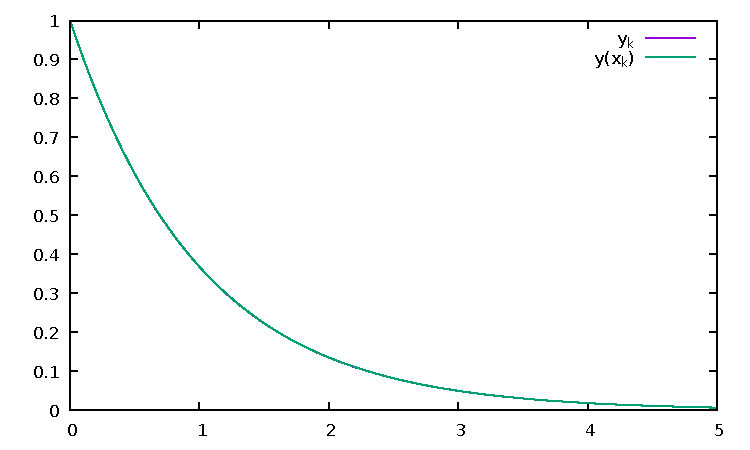
\includegraphics[scale=\SingleImageScale]{12/1Scheme.pdf}
            \caption{Численные значения при $X=5$, $n=100$}
          \end{figure}

    \item Вторая схема аппроксимации
          \[
            \begin{array}{c}
              ((y)_{Y_n})_k=y(x_k)=:y_k         \\
              ((f)_{F_n})_k=f_k:=f(x_k)=-y(x_k) \\
            \end{array}\Rightarrow
            \begin{cases}
              \frac{y_{k+1}-y_{k-1}}{2h}+y_k=0 \\
              y_0=1,\ y_1=1-h
            \end{cases}
          \]
          \begin{enumerate}
            \item Аппроксимацию второго порядка на решении можно проверить, используя теорему выше, но
                  для разнообразия проверим по определению
                  \begin{multline*}
                    \norm{L_h(y)_{Y_h}-f_h}_{F_h}=\max_{k}\left|\frac{y(x_k+h)-y(x_k-h)}{2h}-f(x_k)\right|=\\
                    \left|\begin{array}{c}
                      y(x_k\pm h)=y(x_k)\pm y'(x_k)h + y''(x_k)\frac{h^2}{2}\pm y'''(x_k)\frac{h^3}{6}+\bigO(h^4) \\
                      f(x_k)=y'(x_k) \text{ -- по условию}
                    \end{array}\right| \\
                    =\max_{k}\left|\frac{2hy'(x_k)+\bigO(h^3)}{2h}-y'(x_k)\right| \leq ch^2
                  \end{multline*}
            \item Проверим аппроксимацию на краях $\norm{l_h(y)_h-\varphi_h}_{\Phi_h}$
                  \begin{flalign*}
                    & |y(0)-y_0|=0\leq ch^2 \\
                    & |y(h)-y_1|=|\overbrace{y(0)}^{=1}+y'(0)h+\bigO(h^2)-1+h|=|h\overbrace{(y'(0)+y(0))}^{=0}+\bigO(h^2)|=\leq ch^2
                  \end{flalign*}
            \item Проверим условие нормировки: $\norm{(f)_h-f_h}_{F_h}=|f(x_k)-f(x)|\rightarrow0$
          \end{enumerate}
          Разностная схема имеет второй порядок аппроксимации.
          \[\frac{y_{k+1}-y_{k-1}}{2h}=0\Rightarrow P(\mu)=\mu^2-1\Rightarrow \mu=\pm 1\]
          Схема $\alpha$-устойчива.

          Судя по всей той теории, что описана выше, так как есть $\alpha$-устойчивость, то
          такую разностную схему можно применять для численного подсчета. Давайте попробуем посчитать
          иначе: можем написать решение разностного уравнения второго порядка с постоянными коэффициентами.
          \[\frac{y_{k+1}-y_{k-1}}{2h}+y_k=0\Rightarrow P(\mu)=\frac{\mu^2-1}{2h}+\mu=0\Rightarrow\mu_{1,2}=-h\pm\sqrt{1+h^2}\]
          \[y_k=C_1(-h+\sqrt{1+h^2})^k+C_2(\ \underbrace{-h-\sqrt{1+h^2}}_{<-1}\ )^k\]
          Обратим внимание, что из-за того, что второй корень по модулю больше единицы,
          при большом количестве шагов правое слагаемое в сумме будет доминировать, в результате
          чего решение разностной задачи будет болтаться в зависимости от четности $k$.
          То есть эту схему лучше не применять.
          \begin{figure}[h]
            \centering
            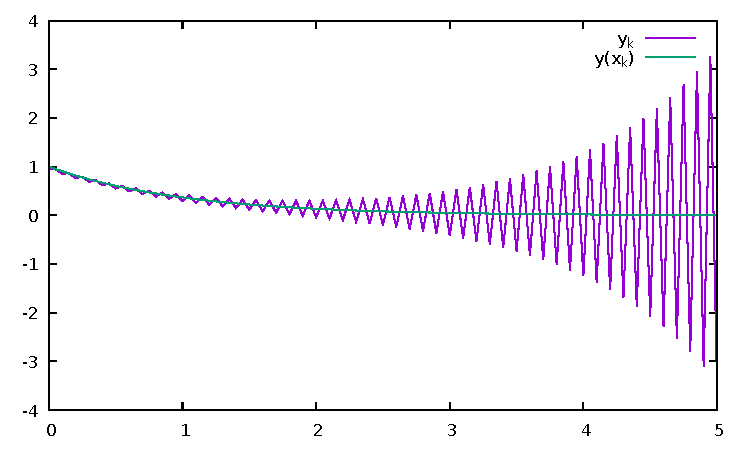
\includegraphics[scale=\SingleImageScale]{12/2Scheme.pdf}
            \caption{Численные значения при $X=5$, $n=100$}
          \end{figure}

    \item Третья схема
          \[
            \begin{cases}
              \frac{y_{k+1}-y_{k-1}}{2h}=-\frac{y_{k+1}+y_{k-1}}{2} \\
              y_0=1,\ y_1=1-h                                       \\
            \end{cases}
          \]

          Аналогично предыщум пунктам проверяется аппроксимация на решении
          2 степени и $\alpha$-устойчивость. Решения разностного уравнения имеют вид
          \[\mu_{1,2}=\pm\sqrt{\frac{1-h}{1+h}},\ \abs{\mu_{1,2}}<1\]

          Заметим, что в данной схеме каждый следующий элемент порождается через предпоследний,
          из-за чего решение задачи будет менять знак в зависимости от $k$.
          Такая схема пригодна для расчетов, но в отличие от первой для нее нужно
          дополнительное краевое условие.
          \begin{figure}[h]
            \centering
            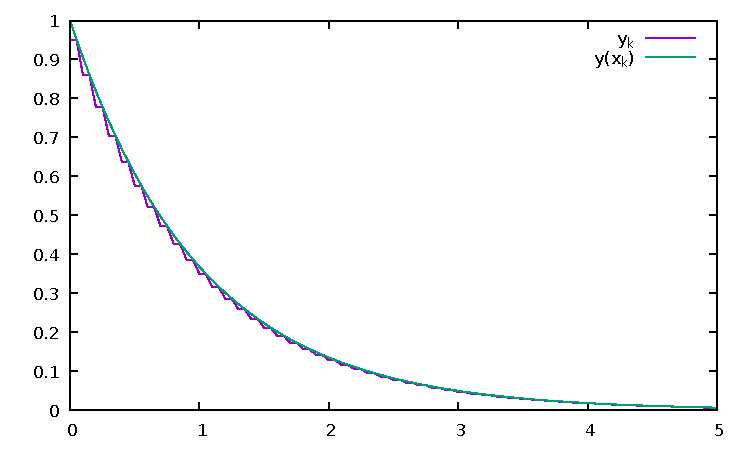
\includegraphics[scale=\SingleImageScale]{12/3Scheme.pdf}
            \caption{Численные значения при $X=5$, $n=100$}
          \end{figure}
  \end{enumerate}
\end{example}


\section{Численные методы решения задачи Коши: метод Тейлора, методы Адамса.}

\subsection*{Метод Тейлора}

Решаем задачу Коши $\begin{cases}
    y'(x)=f(x,y) \\ y(0)=y^0
  \end{cases}$
Мы хотим построить наше решение в точках $y(h),y(2h)\ldots$,
предлагается явно посчитать значения в этих точках,
разложив в ряд Тейлора до $p+1$ степени. Далее для упрощения записи $y\defeq y(x_0),\ f\defeq f(x_0,y(x_0))$:
\[\begin{cases}
    y(x)=y+hy'+\frac{h^2}{2}y''+\sum_{s=2}^{p}y^{(s)}\frac{h^s}{s!}+\bigO(h^{p+1}) \\
    y'=f \text{ -- по условию}                                                     \\
    y''=f_x+f_yy'                                                                  \\
    y'''=f_{xx}+f_{xy}y'+f_{yx}y'+f_{y}y''+f_{yy}(y')^2                            \\
    \cdots
  \end{cases}
\]

Метод применим если $|x-x_0|$ больше области сходимости ряда Тейлора,
иначе предлагается разбивать отрезки на подотрезки и строить решение
в точке $x$ за несколько шагов.

\begin{remark}
  Данный алгоритм может быть полезен, когда требуется решить
  большое количество задач вполне определенного вида с
  различными начальными данными. В этом случае требуемые
  производные можно найти аналитически и сохранить для многократного
  применения.
\end{remark}

\begin{example}
  Решаем задачу $y'(x)=x^2\sin(y(x))$. Мы можем посчитать
  \begin{align*}
    y''(x) & = 2x\sin(y(x))+x^2\cos(y(x))y'(x)      \\
           & = 2x\sin(y(x))+x^4\cos(y(x))\sin(y(x))
  \end{align*}
  Таким образом второй порядок \textit{локальной} точности используя следующую формулу
  \[y_{k+1}=y_k+hx_k^2\sin(y_{k})+\frac{h^2}{2}[2x_k\sin(y_k)+x_k^4\cos(y_k)\sin(y_k)]\]
  Можно продолжать считать производные и получать более точный результат.
\end{example}

\begin{remark}
  Заметим, что здесь нет речи о разностной схеме, так как формально достаточно
  затруднительно посчитать \textit{глобальную} погрешность аппроксимации.
  Если при первом шаге мы считаем производную в известной нам начальной точке,
  то при каждом следующем шаге мы будем искать производную в точке, которая
  никак не привязана к изначальному уравнению.
\end{remark}

\subsection*{Методы Адамса первого порядка точности}

Решаем задачу Коши $\begin{cases}
    y'(x)=f(x,y) \\ y(0)=y^0
  \end{cases}$

Основная идея берется из точного равенства $y'(x_{k+1})\equiv y(x_k)+\int_{x_k}^{x_{k+1}}y'(x)dx=y(x_k)+\int_{x_k}^{x_{k+1}}f(x,y)dx$.
Различные методы Адамса возникают из разных способов взять интеграл

\begin{lemma}
  Пусть $g\in C^k[a,b],\ I(g)=\int_a^bg(x)dx$, тогда
  \begin{flalign*}
    & 1) \abs{I(g)-g(a)(b-a)}\leq \norm{g'}\frac{(b-a)^2}{2} \\
    & 2) \abs{I(g)-g(b)(b-a)}\leq \norm{g'}\frac{(b-a)^2}{2} \\
    & 3) \abs{I(g)-g\left(\frac{a+b}{2}\right)(b-a)}\leq\norm{g''}\frac{(a - b)^3}{24}    \\
    & 4) \abs{I(g)-\frac{g(a)+g(b)}{2}(b-a)}\leq\norm{g''}\frac{(b-a)^3}{12} \\
  \end{flalign*}
\end{lemma}
\begin{proof}
  Первые три неравенства берутся из разложения подынтегральной функции в ряд Тейлора
  с остаточным членом в форме Лагранжа в указанных точках:
  \begin{flalign*}
    & 1) \abs{\int_a^bg(a)+g'(\xi)(x-a)dx-g(a)(b-a)}=\abs{\int_a^bg'(\xi)(x-a)dx}\leq\norm{g'}\int_a^b(x-a)dx\leq\norm{g'}\frac{(b-a)^2}{2} \\
    & 2) \abs{\int_a^bg(b)+g'(\xi)(x-b)dx-g(b)(b-a)}=\abs{\int_a^bg'(\xi)(x-b)dx}\leq\norm{g'}\int_a^b(b-x)dx\leq\norm{g'}\frac{(b-a)^2}{2}                 \\
    & 3) \abs{\int_a^bg\left(\frac{a+b}{2}\right)+g'\left(\frac{a+b}{2}\right)\left(x-\left(\frac{a+b}{2}\right)\right)+\frac{g''(\xi)}{2}\left(x-\left(\frac{a+b}{2}\right)\right)^2dx-g\left(\frac{a+b}{2}\right)(b-a)}=    \\
    & \: \abs{\int_a^bg\left(\frac{a+b}{2}\right)dx+\underbrace{\int_a^bg'\left(\frac{a+b}{2}\right)\left(x-\left(\frac{a+b}{2}\right)\right)dx}_{=\ 0,\ (\text{симм. отн. середины})}+\int_a^b\frac{g''(\xi)}{2}\left(x-\left(\frac{a+b}{2}\right)\right)^2dx-g\left(\frac{a+b}{2}\right)(b-a)} \\
    & = \abs{\int_a^b\frac{g''(\xi)}{2}\left(x-\left(\frac{a+b}{2}\right)\right)^2dx}\leq \frac{\norm{g''}}{2}\abs{\int_a^b\left(x-\left(\frac{a+b}{2}\right)\right)^2dx}=\norm{g''}\frac{(a - b)^3}{24}
  \end{flalign*}
  Для доказательства 4ого пункта рассматриваем следующий интеграл
  \begin{multline*}
    \frac{1}{2}\int_a^bg''(x)(x-a)(x-b)dx= \frac{1}{2}g'(x)(x-a)(x-b)|_a^{b}-\frac{1}{2}\int_a^bg'(x)((x-b)+(x-a))dx= \\
    = -\frac{1}{2}g(x)((x-b)+(x-a))|_a^b +\int_a^bg(x)dx=\int_a^bg(x)dx-\frac{g(a)+g(b)}{2}(b-a)
  \end{multline*}
  Доказали эквивалентность предложенного интеграла, оценим его:
  \[\abs{\frac{1}{2}\int_a^bg''(x)(x-a)(x-b)dx}\leq\frac{\norm{g''}}{2}\abs{\int_a^bg''(x)(x-a)(x-b)dx}\leq\frac{\norm{g''}}{12}(b-a)^3\]
\end{proof}

\subsubsection*{Явный метод Эйлера}
Разностная схема получается из пункта 1) доказанной выше леммы:
\[\frac{y_{k+1}-y_k}{h}= f(x_k,y_k) + \bigO(h),\ y_0=y(x_0)\]
Локальная погрешность $O(h^2)$, глобальная погрешность и сходимость $O(h)$.

\subsubsection*{Неявный метод Эйлера}
Разностная схема получается из пункта 2) доказанной выше леммы:
\[\frac{y_{k+1}-y_k}{h}= f(x_{k+1},y_{k+1}) + \bigO(h),\ y_0=y(x_0)\]
Локальная погрешность $O(h^2)$, глобальная погрешность и сходимость $O(h)$.
Является более устойчивой схемой, чем явный метод Эйлера.

Неявный метод называется именно так из-за того, что разностное уравнение
в схеме является нелинейным. Для того, чтобы его решать предлагается
вводить внутренний итерационный процесс
\[y_{k+1}^{j+1}= y_k+hf(x_{k+1},y_{k+1}^{j}),\ y_{k+1}^{0}=y_{k}\]
При достаточно малых $h$ и достаточно гладкой $f$ можно показать,
что данное отображение является сжимающим.

\subsection*{Методы Адамса второго порядка точности}

\subsubsection*{Через формулу прямоугольника по средней точке}
Из пункта 3) доказанной выше леммы получили следующую оценку
\[y(x_k+h)=y(x_k)+hf(y(x_k+h/2), x_k+h/2)+\bigO(h^3)\]
Но в пространстве $Y_h$ не определен узел $x_k+h/2$, поэтому
для расчетной формулы нужно думать что-то другое.

Один из вариантов: представить $y(x_k+h/2):=\frac{y(x_k)+y(x_k+h)}{2}$ и
воспользоваться снова итерационным процессом для расчетной
формулы $y_{k+1}=y_{k}+hf(\frac{y_k+y_{k+1}}{2}, x_k+h/2)+\bigO(h^3)$.

Рассмотрим другой вариант: пусть $\exists\ y_{k+1/2}^*\defeq y_k+\bigO(h^2)$, тогда
мы можем записать расчетную формулу следующим образом:
\begin{multline*}
  y_{k+1}=y_{k}+hf(y_k, x_k+h/2)\pm hf(x_k+h/2,y_{k+1/2}^*)+\bigO(h^3)= \\
  = y_{k}+hf(x_k+h/2,y_{k+1/2}^*)+ (hf(y_k, x_k+h/2)-hf(x_k+h/2,y_{k+1/2}^*))+\bigO(h^3)
\end{multline*}
Воспользуемся теоремой о среднем: $\tilde{y_k}$ - точка между $y_{k+1/2}^*$ и $y_k$
\[y_{k+1}= y_{k}+hf(x_k+h/2,y_{k+1/2}^*)+ \frac{h}{2}(f_x(\tilde{y_k}, x_k+h/2))\underbrace{(y_{k+1/2}^*-y_k)}_{\bigO(h^2)}+\bigO(h^3)=y_{k}+hf(x_k+h/2,y_{k+1/2}^*)+\bigO(h^3)\]
Точку $y_{k+1/2}^*$ можно посчитать с помощью явного метода Эйлера,
который как раз и обеспечивает второй порядок сходимости $y_{k+1/2}^*=y_k+\frac{h}{2}f(x_k,y_k)$
Итоговая расчетная форумла
\[\begin{cases}
    y_{k+1/2}^*=y_k+\frac{h}{2}f(x_k,y_k) \\
    y_{k+1}=y_{k}+hf(x_k+h/2,y_{k+1/2}^*) \\
    y_0=y(x_0)
  \end{cases}\]

\subsubsection*{Через формулу трапеции}
Разностная схема получается из пункта 4) доказанной выше леммы:
\[y_{k+1}=y_k+h\frac{f(x_k,y_k)+f(x_{k+1},y_{k+1})}{2}+\bigO(h^3)\]
Схема получается нелинейная, для решения можно воспользоваться итерационным
методом. Мы воспользуемся аналогично формуле прямоугольника по центральной
точке хитростью.

Пусть $\exists\ y_{k+1}^*\defeq y_k+\bigO(h^2)$, тогда
мы можем записать расчетную формулу следующим образом:
\begin{multline*}
  y_{k+1}=y_k+h\frac{f(x_k,y_k)+f(x_{k+1},y_{k+1})}{2}\pm\frac{h}{2}f(x_{k+1},y_{k+1}^*)+\bigO(h^3)= \\
  = y_k+h\frac{f(x_k,y_k)+f(x_{k+1},y_{k+1}^*)}{2}+\frac{h}{2}(f(x_{k+1},y_{k+1})-f(x_{k+1},y_{k+1}^*))+\bigO(h^3)
\end{multline*}
Воспользуемся теоремой о среднем: $\tilde{y_k}$ - точка между $y_{k+1}^*$ и $y_k$
\begin{multline*}
  y_{k+1}=y_k+h\frac{f(x_k,y_k)+f(x_{k+1},y_{k+1}^*)}{2}+\frac{h}{2}f_x(x_{k+1},\tilde{y_k})\underbrace{(y_{k+1}^*-y_k)}_{\bigO(h^2)}+\bigO(h^3)= \\
  =y_k+h\frac{f(x_k,y_k)+f(x_{k+1},y_{k+1}^*)}{2}+\bigO(h^3)
\end{multline*}
Точку $y_{k+1}^*$ будем искать с помощью явного метода Эйлера $y_{k+1}^*=y_k+hf(x_k,y_k)$.
Итоговая расчетная формула
\[\begin{cases}
    y_{k+1}^*=y_k+hf(x_k,y_k)                                         \\
    y_{k+1}=y_k+h\frac{f(x_k,y_k)+f(x_{k+1},y_{k+1}^*)}{2}+\bigO(h^3) \\
    y_0=y(x_0)
  \end{cases}\]
\begin{remark}
  Предложенные варианты с заменой на явные методы Эйлера облегчают
  подсчет итоговой расчетной формулы, но при этом отрицательно влияют на Устойчивость
  задачи.
\end{remark}

\section{Методы Рунге–Кутта для решения задачи Коши.}

\section{Вычисление главного члена погрешности для простейших схем для задачи Коши. Оценка глобальной погрешности явного одношагового метода.}

\section{Устойчивые и неустойчивые задачи. Жесткие системы.}

\section{Метод Лебедева решения жестких систем.}

\section[Обыкновенные дифференциальные уравнения второго порядка, аппроксимация, alpha-устойчивость. Аппроксимация краевых условий третьего рода.]{Обыкновенные дифференциальные уравнения второго порядка, аппроксимация, $\alpha$-устойчивость. Аппроксимация краевых условий третьего рода.}

\subsection*{Обыкновенные дифференциальные уравнения второго порядка}

\begin{definition}
  Будем рассматривать только задачи с правыми
  частями, не зависящими от $y'$: $f(x,y,y')=f(x,y)$.
  вида
  \begin{equation}\label{eq:second_cauchy:task}
    y''=f(x,y)
  \end{equation}
  Для такой задачи предлагается строить следующую разностную схему
  \begin{equation}\label{eq:second_cauchy:recur_scheme}
    \begin{array}{c}
      h=\frac{X}{N},\ x_i=x_o+i\cdot h,\ y_h=\{y_i\}_{i=0}^{N},\ \norm{y_h}_{Y_h}=\max\limits_{i}\abs{y_k} \\
      \begin{cases}
        \frac{1}{h^2}\sum_{i=0}^na_{-i}y_{k-i}=\sum_{i=0}^nb_{-i}f_{k-i},\ k=n,n+1\ldots \\
        y_0,y_1,\ldots,y_{n-1} - \text{ начальные условия}
      \end{cases}                                                                            \\
    \end{array}
  \end{equation}
  где $a_{-i}$, $b_{-i}$ не зависят от $h$, $a_0$, $a_n$ $\neq0$ и $f_{k-i}=f(x_{k-i},y_{k-i})$.
\end{definition}

Хотим для такой разностной схемы проверять условие аппроксимации на решении,
чтобы далее пользоваться теоремой Филиппова. Зададим функцию погрешности
\[r^k_h\defeq\frac{1}{h^2}\sum_{i=0}^na_{-i}y(x_{k-i})-\sum_{i=0}^nb_{-i}f(x_{k-i},y(x_{k-i}))\]

Условия аппроксимации на решении с порядком $p$ на отрезке $[x_0,x_0+X]$:
$\begin{cases}\norm{r_h}_{F_h}\leq ch^p \\
    \norm{f_h-(f)_h}_{F_h}\underset{h\rightarrow0}{\rightarrow}0
  \end{cases}$

Коэффициенты в общем случае $a_{-i}$ и $b_{-i}$ находятся из условий
аппроксимации на задаче
\[\norm{L_h(y)_{Y_h} - (Ly)_{F_h}}_{F_h}+\norm{(f)_{F_h}-f_h}_{F_h}\leq c_1h^{p_1}\]

\begin{theorem}[Необходимые и достаточные условия аппроксимации на решении]
  Для задачи \eqref{eq:second_cauchy:task} с разностной схемой \eqref{eq:second_cauchy:recur_scheme}
  необходимые и достаточные условия аппроксимации на решении имеют вид
  \[\sum_{i=0}^na_{-i}=0;\ \sum_{i=0}^nb_{-i}=1;\ \sum_{i=0}^na_{-i}i=0;\sum_{i=0}^ni^2a_{-i}=2\]
\end{theorem}
\begin{proof}
  \begin{enumerate}
    \item Проверим условие нормировки правых частей
          \[\norm{f_h-(f)_h}_{F_h}=\norm{f(x_{k-i})-\sum_{i=0}^nb_{-i}f(x_{k-i})}_{F_h}=\norm{f(x_{k-i})\left(1-\sum_{i=0}^nb_{-i}\right)}_{F_h}\underset{h\rightarrow0}{\rightarrow}0\Leftrightarrow\sum_{i=0}^nb_{-i}=1\]
    \item Выпишем ряд Тейлора для левой и правой части в узлах $\{x_k\}$:
          \begin{align*}
            y(x_k-ih)=y(x_k)-ihy'(x_k)+\frac{(ih)^2}{2}y''(x_k) + \bigO(h^3) \\
            f(x_k-ih)=y''(x_k-ih)=y''(x_k)-ihy'''(x_k) + \bigO(h^2)          \\
          \end{align*}
          Запишем условие аппроксимации на решении:
          \begin{multline*}
            \abs{\frac{1}{h^2}\sum_{i=0}^na_{-i}y_{k-i}-\sum_{i=0}^nb_{-i}f(x_k-ih)} \\
            = \left|\frac{1}{h^2}\sum_{i=0}^na_{-i}y(x_k)+\frac{1}{h^2}\sum_{i=0}^na_{-i}(-ihy'(x_k))+\frac{1}{h^2}\sum_{i=0}^na_{-i}\left(\frac{(ih)^2}{2}y''(x_k)\right)
            -\sum_{i=0}^nb_{-i}y''(x_k)+\bigO(h)\right|\leq
          \end{multline*}
          \[ \leq\abs{\frac{y(x_k)}{h^2}\sum_{i=0}^na_{-i}+\frac{y'(x_k)}{h}\left(-\sum_{i=0}^na_{-i}i\right)+y''(x_k)\left(\sum_{i=0}^na_{-i}\frac{i^2}{2}-\sum_{i=0}^nb_{-i}\right)+\bigO(h)}\leq ch \]
          Для выполнения условия аппроксимации нужно, чтобы все коэффициенты до $h$ занулились, отсюда
          и из проверки нормировки следует доказательство теоремы.
  \end{enumerate}
\end{proof}
\begin{remark}
  Для того, чтобы найти $a_{-i}$ и $b_{-i}$ надо решить систему уравнений.
  Для того, чтобы система была разрешима, важно проверить $p=2n$.
\end{remark}

\subsection*{$\alpha$-устойчивость задачи второго порядка}

В случае задачи \eqref{eq:second_cauchy:task} проверяют
более слабое определение $\alpha$-устойчивости.

\begin{definition}
  Для задачи Коши $y''=f(x)$ схема называется $\alpha$-
  устойчивой, если все корни соответствующего характеристического
  многочлена $\sum_{i=0}^na_{-i}\mu^{k-i}$ однородного уравнения
  принадлежат единичному кругу и на границе круга нет кратных корней, за
  исключением $\mu=1$ кратности $2$.
\end{definition}

Отличие условия устойчивости для задачи Коши второго порядка
от условия устойчивости для задачи первого порядка обусловлено
более высокой степенью $h$ в правой части разностной схемы $\sum_{i=0}^na_{-i}y_{k-i}=h^2\sum_{i=0}^nb_{-i}f_{k-i}$.

\subsection*{Аппроксимация граничных условий третьего рода}
Пусть дана задача
\[\begin{cases}
    -(k(x)y')'+p(x)y=f(x),\ 0<k_0<k(x)<k_1,\ 0\leq p(x)\leq p_1 \\
    ay+by'=c
  \end{cases}\]
Предлагается выбрать следующую разностную схему
\[-\frac{1}{h}\left[k(x_{i+1/2})\frac{y_{i+1}-y_i}{h}-k(x_{i-1/2})\frac{y_{i}-y_{i-1}}{h}\right]+p(x_i)y_i=f_i\]
Проверим, что она второго порядка аппроксимации на решении:
\[\abs{-\frac{1}{h}\underbrace{\left[k\left(x_k+\frac{h}{2}\right)\frac{y(x_k+h)-y(x_k)}{h}-k\left(x_k-\frac{h}{2}\right)\frac{y(x_k)-y(x_k-h)}{h}\right]}_{\star}+p(x_k)y(x_k)-f(x_k)}\leq ch^2\]
Напомним формулу разложения в ряд Тейлора в точке $x_k$
\[u(x\pm h)=u(x)\pm hu'(x)+\frac{h^2}{2}u''(x)+\bigO(h^3)\]
Отдельно решим то, что помечено $\star$:
\begin{multline*}
  \left(k(x_k)+\frac{h}{2}k'(x_k)+\frac{h^2}{8}k''(x_k)+\bigO(h^3)\right)\left(y'(x_k)+\frac{h}{2}k''(x_k)+\bigO(h^2)\right)- \\
  \left(k(x_k)-\frac{h}{2}k'(x_k)+\frac{h^2}{8}k''(x_k)+\bigO(h^3)\right)\left(y'(x_k)-\frac{h}{2}k''(x_k)+\bigO(h^2)\right)=
\end{multline*}
\[=hk'(x_k)y'(x_k)+hk(x_k)y''(x_k)+\bigO(h^3)=h(k(x_k)y'(x_k))'+\bigO(h^3)\]
Подставим получившееся значение и начальное условие в изначальное уравнение:
\[\abs{-(k(x_k)y'(x_k))'+\bigO(h^2)+p(x_k)y(x_k)-(-(k(x_k)y'(x_k))'+p(x_k)y(x_k))}\leq ch^2\]
Действительно, предложенная схема обладает вторым порядком аппроксимации на решении.

Построим для краевого условия задачи - краевого условия \textit{третьего рода} -
конечно-разностную аппроксимацию второго порядка точности на решении,
используя значения функции $y$ в точках $x_0=0$ и $x_1=h$.
Для простоты возьмем $k(x)\equiv1$. Воспользуемся $\delta$-поправкой.

Хотим получить следующее:
\[\abs{ay(0)+b\frac{y(h)-y(0)}{h}-c-\delta}\leq ch^2\]

Из формулы Тейлора в точке $0$ имеем:
\[\abs{ay(0)+b\frac{y(0)+hy'(0)+\frac{h^2}{2}y''(0)+\bigO(h^3)-y(0)}{h}-c-\delta}\leq ch^2\]
\[\abs{ay(0)+by'(0)+\frac{bh}{2}y''(0)+\bigO(h^2)-c-\delta}\leq ch^2\]
\[\abs{ay(0)+by'(0)+\frac{bh}{2}(p(0)y(0)-f(0))+\bigO(h^2)-c-\delta}\leq ch^2\]
Чтобы достигалось соответствующее неравенство
требуется взять $\delta:=\frac{bh}{2}(p(0)y(0)-f(0))$.

Таким образом аппроксимация второго порядка на краевом условии имеет вид
\[ay_0+b\frac{y_1-y_0}{h}=c+\frac{bh}{2}(p(0)y_0-f(0))\]

\subsection*{Примеры}
Рассмотрим разностные схемы для уравнения $y''(x)=f(x)$
\begin{example}
  Естественная аппроксимация:
  \[\frac{y_{i+1}-2y_i+y_{i-1}}{h^2}=f_k\]
  Главный член погрешности на решении равен
  \[r_h:=L_h(y)_h-f_h=\frac{h^2}{12}y^{(4)}(x_k)+\bigO(h^4)\]
\end{example}
\begin{example}
  Схема
  \[\frac{y_{i+1}-2y_i+y_{i-1}}{h^2}=f_k\frac{h^2}{12}f''(x_k)\]
  аппроксимирует уравнение на решении с порядком $\bigO(h^4)$
  (см. предыдущий пример и пользуемся тем, что $y''=f$).
\end{example}
\begin{example}
  Схема Нумерова
  \[\frac{y_{i+1}-2y_i+y_{i-1}}{h^2}=\frac{f_{k+1}+10f_k+f_{k-1}}{12}\]
  Главный член погрешности имеет вид
  \[r_h:=L_h(y)_h-f_h=\frac{h^2}{12}y^{(4)}(x_k)+\frac{h^4}{360}y^{(6)}(x_k)-\frac{h^2}{12}f^{(2)}(x_k)-\frac{h^4}{144}f^{(4)}(x_k)=-\frac{h^4}{240}y^{(6)}(x_k)+\bigO(h^6)\]
  Такую схему используют, если невозможно посчитать $f''$.
\end{example}

\section{Устойчивость краевой задачи для уравнения второго порядка: метод собственных функций.}

\section{Устойчивость краевой задачи для уравнения второго порядка: энергетический метод.}

Напомним определение устойчивости
\begin{definition}
  Разностная схема $\begin{cases}
      L_hy_h = f_h \\
      l_hy_h = \varphi_h
    \end{cases}$
  называется устойчивой, если:
  $\forall y_h^{(1)}$, $y_h^{(2)}\ \forall \varepsilon > 0\ \exists\delta=\delta(\varepsilon):$
  \[\norm{f^{(1)}_h-f^{(2)}_h}+\norm{\varphi^{(1)}_h-\varphi^{(2)}_h}\leq\delta,\ \forall h\leq h_0\Rightarrow\norm{y^{(1)}_h-y^{(2)}_h}\leq\varepsilon\]
\end{definition}
\begin{definition}
  Линейная схема $\begin{cases}
      L_hy_h = f_h \\
      l_hy_h = \varphi_h
    \end{cases}$
  называется устойчивой, если:
  \[\norm{y^{(1)}_h-y^{(2)}_h}\leq C\left(\norm{f^{(1)}_h-f^{(2)}_h}+\norm{\varphi^{(1)}_h-\varphi^{(2)}_h}\right),\ \forall h\leq h_0\]
  $C$ не должна зависеть от $h$.
\end{definition}

Будем доказывать устойчивость разностной схемы энергетическим методом.
Запишем нашу дифференциалную задачу
\[-y''(x)+p(x)y(x)=f(x),\ y(0) = y'(1) = 0,\ p(x)\geq 0\]
Умножим уравнение на $y(x)$, и результат проинтегрируем по отрезку $[0, 1]$
\[\int_0^1 (-y''y+py^2)dx = \int_0^1fydx \]
\[\int_0^1 -y''ydx+ \int_0^1py^2 dx = \int_0^1fydx \]
Проинтегрируем по частям первое слагаемое
\[\int_0^1 -y''ydx = \int_0^1-ydy' = -yy'\vert^1_0 - \int_0^1y'd(-y) = \int_0^1(y')^2dx\]
Получили интегральное тождество
\[\int_0^1 (y'(x))^2dx+ \int_0^1py^2 dx = \int_0^1fydx \]
Оценим слева через неравенство, связывающее интегралы от квадратов
функции и ее производной. Так как $y(0) = 0$, то справедливо следующее:
\[y(x_0) = \int_0^{x_0}y'(x)dx\]
Применим интегральную форму неравенства Коши-Буняковского:
\[|y(x_0)|^2 = \left|\int_0^{x_0}y'dx\right|^2\leq\left(\int_0^{x_0}1^2dx\right)\left(\int_0^{x_0}(y')^2dx\right)\leq\int_0^{x_0}(y')^2dx\leq\int_0^{1}(y')^2dx\]
После интегрирования по $x_0$ по отрезку $[0,1]$ обеих частей получим искомое равенство
\[\int_0^1|y(x_0)|^2dx_0 \leq \int_0^{1}(y')^2dx\int_0^1dx_0 \Leftrightarrow \int_0^1y^2dx\leq\int_0^1(y')^2dx\]
Оценку справа выведем из разности квадратов:
\[0\leq\int_0^1(f - y)^2dx\leq\int_0^1f^2dx-2\int_0^1fydx+\int_0^1y^2dx\]
\[\Rightarrow\int_0^1fydx\leq\frac{1}{2}\left(\int_0^1f^2dx + \int_0^1y^2dx\right)\]

Таким образом, имеем:
\[\int_0^1y^2dx\leq\int_0^1 (y'(x))^2dx+ \int_0^1py^2 dx = \int_0^1fydx\leq\frac{1}{2}\left(\int_0^1f^2dx + \int_0^1y^2dx\right)\]
Получаем следующую оценку
\[\int_0^1y^2dx\leq\int_0^1f^2dx\Rightarrow\Vert y\Vert_{L_2(0,1)}\leq\Vert f\Vert_{L_2(0,1)}\]
Это означает устойчивость дифференциальной задачи по правой части.

Докажем теперь устойчивость разностной схемы.
\[-\frac{y_{k+1}-2y_k+y_{k-1}}{h^2}+p_ky_k = f_k,\ 1 \leq k \leq N-1,\ y_0 = 0,\ y_N = y_{N-1}\]
Умножим на $y_k$ и просуммируем от $1$ до $N-1$. Так как $y_0 = 0,\ y_N = y_{N-1}$
\[-\frac{1}{h^2}\left(\sum_{k=1}^{N-1}\left(y_{k+1}-2y_k+y_{k-1}\right)y_k\right)=-\frac{1}{h^2}\left(\sum_{k=1}^{N-1}\left(y_{k+1}-y_k-y_k+y_{k-1}\right)y_k\right)=\]
\[=-\frac{1}{h^2}\sum_{k=1}^{N-1}\left(y_{k+1}-y_k\right)y_k+\frac{1}{h^2}\sum_{k=1}^{N-1}\left(y_k-y_{k-1}\right)y_k=-\frac{1}{h^2}\sum_{k=2}^{N}\left(y_{k}-y_{k-1}\right)y_{k-1}+\frac{1}{h^2}\sum_{k=1}^{N-1}\left(y_k-y_{k-1}\right)y_k=\]
\[=-\frac{1}{h^2}\sum_{k=2}^{N}\left(-\left(y_{k}-y_{k-1}\right)y_{k-1}+\left(y_k-y_{k-1}\right)y_k\right)=\frac{1}{h^2}\sum_{k=1}^{N}(y_k-y_{k-1})^2\]
Получили конечномерный аналог интегрального тождества:
\[\frac{1}{h^2}\sum_{k=1}^N(y_k-y_{k-1})^2+\sum_{k=1}^{N-1}p_ky_k^2=\sum_{k=1}^{N-1}f_ky_k\]
Для оценки слева докажем сеточный аналог неравенства для функции и ее производной в точках $k=1,...,N-1$.
Так как $y_0 = 0$, справедливо следующее:
\[y_k=\sum_{i=1}^{k}(y_i-y_{i-1})\]
Воспользуемся неравенством Коши-Буняковского и $y_N=y_{N-1}$
\[y_k^2\leq\left(\sum_{i=1}^k1^2\right)\left(\sum_{i=1}^k(y_i-y_{i-1})^2\right)\leq (N-1)\sum_{i=1}^{N-1}(y_i-y_{i-1})^2\]
Суммируя до $N-1$ обе части, при $h=\frac{2}{2N-1}$ получаем оценку:
\[\sum_{k=1}^{N-1}y_k^2\leq(N-1)^2\sum_{k=1}^{N-1}(y_k-y_{k-1})^2\leq\frac{1}{h^2}\sum_{k=1}^{N-1}(y_k-y_{k-1})^2\]
Найдем аналогично дифференциальному неравенству оценку справа
\[0\leq\sum_{k=1}^{N-1}(f_k-y_k)^2 = \sum_{k=1}^{N-1}f_k^2-2\sum_{k=1}^{N-1}f_ky_k+\sum_{k=1}^{N-1}y_k^2\]
\[\Rightarrow\sum_{k=1}^{N-1}f_ky_k\leq\frac{1}{2}\left(\sum_{k=1}^{N-1}f_k^2+\sum_{k=1}^{N-1}y_k^2\right)\]
Итоговая оценка имеет вид
\[\sum_{k=1}^{N-1}y_k^2\leq\frac{1}{h^2}\sum_{k=1}^{N-1}(y_k-y_{k-1})^2+\sum_{k=1}^{N-1}p_ky_k^2=\sum_{k=1}^{N-1}f_ky_k\leq\frac{1}{2}\left(\sum_{k=1}^{N-1}f_k^2+\sum_{k=1}^{N-1}y_k^2\right)\]
Таким образом,
\[\sum_{k=1}^{N-1}y_k^2\leq\sum_{k=1}^{N-1}f_k^2\Rightarrow\sum_{k=1}^{N-1}y_k^2h\leq\sum_{k=1}^{N-1}f_k^2h\Rightarrow\Vert y_h\Vert^2_h\leq\Vert f_h\Vert^2_h\]
То есть \textbf{разностная схема устойчива} в норме $\Vert\cdot\Vert_h$.


\section{Метод прогонки.}

Требуется найти решение $y$ задачи $Ay=f,\ A\in \mathbb{R}^{N-1\times N-1}$
с заданной матрицей квадратной матрицей $A$ (примеры см. ниже), заданной правой частью $f$.

Перепишем матрицу $A$, сделав вспомогательные замены:
\[\left(\begin{array}{cccccc}
      c_1  & -b_1 &        &          &          & 0        \\
      -a_2 & c_2  & -b_2   &          &          &          \\
           &      & \cdots & \cdots   &          &          \\
           &      &        & -a_{N-2} & c_{N-2}  & -b_{N-2} \\
      0    &      &        &          & -a_{N-1} & c_{N-1}  \\
    \end{array}\right)\]
Тогда задачу можно переписать следующем образом
\begin{equation}\label{eq:tridiag_method}
  \begin{array}{cc}
    c_1y_1-b_1y_2=f_1,                      & k=1            \\
    -a_ky_{k-1}+c_ky_k-b_ky_{k+1}=f_k       & k=2,\ldots,N-2 \\
    -a_{N-1}y_{N-2}+c_{N-1}y_{N-1}=f_{N-1}, & k=N-1
  \end{array}
\end{equation}

Перепишем первое уравнение
\[ c_1y_1-b_1y_2=f_1 \Leftrightarrow y_1-\frac{b_1}{c_1}y_2=\frac{f_1}{c_1}\Leftrightarrow y_1=\alpha_2y_2+\beta_2,\ \alpha_2=\frac{b_1}{c_1},\ \beta_2=\frac{f_1}{c_1}\]
Найдем $\alpha_{k+1}$ и $\beta_{k+1}$, используя полученную формулу $y_{k-1}=\alpha_ky_k+\beta_k$, подставив во второе уравнение
\[-a_k(\alpha_ky_k+\beta_k)+c_ky_k-b_ky_{k+1}=f_k\Leftrightarrow(-a_k\alpha_k+c_k)y_k-a_k\beta_k-b_ky_{k+1}=f_k\Leftrightarrow\]
\[\Leftrightarrow(-\alpha_ka_k+c_k)y_k+(-b_k)y_{k+1}=a_k\beta_k+f_k\Leftrightarrow y_k=\left(\frac{b_k}{c_k-\alpha_ka_k}\right)y_{k+1}+\frac{a_k\beta_k+f_k}{c_k-\alpha_ka_k}\]
\[\alpha_{k+1}=\frac{b_k}{c_k-\alpha_ka_k},\ \beta_{k+1}=\frac{a_k\beta_k+f_k}{c_k-\alpha_ka_k}\]
Рассмотрим последнее равенство, подставим в него $y_{N-2}=\alpha_{N-1}y_{N-1}+\beta_{N-1}$
\[-a_{N-1}(\alpha_{N-1}y_{N-1}+\beta_{N-1})+c_{N-1}y_{N-1}=f_{N-1}\]
\[y_{N-1}=\frac{f_{N-1}+a_{N-1}\beta_{N-1}}{c_{N-1}-a_{N-1}\alpha_{N-1}};\ y_k=\alpha_{k+1}y_{k+1}+\beta_{k+1},\ k=N-2,\ldots,1\]
Получили формулы для \textit{правой прогонки}.

\begin{theorem}[Достаточные условия корректности и устойчивости метода прогонки]
  Пусть коэффициенты \eqref{eq:tridiag_method} действительны и удовлетворяют
  условиям: $c_1$, $c_{N-1}$, $a_k$, $c_k$, $b_k$ при $k=2,\ldots,N-2$
  отличны от нуля и
  \[\abs{c_k}\geq\abs{a_k}+\abs{b_k},\ k=2,\ldots,N-2\]
  \[\abs{c_1}\geq\abs{b_1};\ \abs{c_{N-1}}\geq\abs{a_{N-1}}\]
  При чем хотя бы одно из неравенств является строгим. Тогда
  для формул метода прогонки справедливы неравенства
  \[c_k-a_k\alpha_k\neq0,\ \abs{a_k}\leq1,\ k=2,\ldots,N-1\]
  гарантирующие разрешимость и устойчивость, то есть корректность метода.
\end{theorem}
\begin{proof}
  Убедимся методом индукции, что ни один из знаменателей не обращается в ноль,
  то есть убедимся в устойчивости метода.
  База: $\abs{\frac{b_1}{c_1}}=\abs{\alpha_2}\leq1$ из условий теоремы.
  Шаг: Пусть $\abs{\alpha_k}\leq1$.
  \[\abs{c_k-a_k\alpha_k}\geq\abs{c_k}-\abs{a_k}\abs{\alpha_k}\geq\abs{c_k}-\abs{\alpha_k}\geq\abs{b_k}>0\]
  \[\Rightarrow\abs{\alpha_{k+1}}=\frac{\abs{b_k}}{\abs{c_k-\alpha_ka_k}}\leq1\]
  Обратим внимание, что если $\abs{\alpha_{k_0}}<1$, то $\forall k>k_0$ $\alpha_k<1$.

  Проверим, что последнее слагаемое так же не обратится в ноль. Рассмотрим
  \[\abs{c_{N-1}-\alpha_{N-1}a_{N-1}}\geq\abs{c_{N-1}}-\abs{\alpha_{N-1}}\abs{a_{N-1}}\]
  Здесь нам потребуется условие, что хотя бы одно из неравенств должно обращаться в строгое равенство.
  \begin{enumerate}
    \item Если $\abs{c_{N-1}}>\abs{a_{N-1}}$, то $\abs{c_{N-1}}-\abs{\alpha_{N-1}}\abs{a_{N-1}}>0$, значит и $\abs{c_{N-1}-\alpha_{N-1}a_{N-1}}>0$, ч.т.д.
    \item Если $\abs{c_k}>\abs{a_k}+\abs{b_k}$, то $\abs{c_k}-\abs{a_k}>\abs{b_k}>0$, значит и $\abs{c_{N-1}-\alpha_{N-1}a_{N-1}}>0$, ч.т.д.
    \item Если $\abs{c_1}>\abs{b_1}$, то $\abs{\alpha_2}<1\Rightarrow\abs{\alpha_{N-1}<1}$, значит и $\abs{c_{N-1}-\alpha_{N-1}a_{N-1}}>0$, ч.т.д.
  \end{enumerate}
\end{proof}

\begin{example}
  Для задачи $-y''=f,\ y(0)=a,\ y(1)=b$ разностная аппроксимация имеет вид
  \[\frac{1}{h^2}\underset{N-1\times N-1}{\left(\begin{array}{cccccc}
        2  & -1 &        &        &    & 0  \\
        -1 & 2  & -1     &        &    &    \\
           &    & \cdots & \cdots &    &    \\
           &    &        & -1     & 2  & -1 \\
        0  &    &        &        & -1 & 1  \\
      \end{array}\right)}
    \left(\begin{array}{c}
        y_{1}   \\
        \\
        \vdots  \\
        \\
        y_{N-1} \\
      \end{array}\right)
    =\left(\begin{array}{c}
        f_{1} +\frac{a}{h^2}   \\
        \\
        \vdots                 \\
        \\
        f_{N-1} +\frac{b}{h^2} \\
      \end{array}\right)
  \]
  В данном примере мы исключили известные значениея $y_0$, $y_N$. Метод прогонки устойчив.
\end{example}

\begin{example}
  Для задачи $-y''=f,\ y'(0)=a,\ y'(1)=b$ разностная аппроксимация имеет вид
  \[\frac{1}{h^2}\underset{N+1\times N+1}{\left(\begin{array}{cccccc}
        2  & -2 &        &        &    & 0  \\
        -1 & 2  & -1     &        &    &    \\
           &    & \cdots & \cdots &    &    \\
           &    &        & -1     & 2  & -1 \\
        0  &    &        &        & -2 & 2  \\
      \end{array}\right)}
    \left(\begin{array}{c}
        y_{0}  \\
        \\
        \vdots \\
        \\
        y_{N}  \\
      \end{array}\right)
    =\left(\begin{array}{c}
        f_{0} -\frac{2a}{h} \\
        \\
        \vdots              \\
        \\
        f_{N} -\frac{2b}{h} \\
      \end{array}\right)
  \]
  Аппроксимация для краевых условий здесь подобрана с помощью $\delta$-поправки.
  Метод прогонки в данной задаче не устойчив, так как не выполняется условие
  о наличии хотя бы одного строгого неравенства.
\end{example}

\section{Метод стрельбы и метод Фурье. Численные методы линейной алгебры.}

\section{Нормы векторов, линейных операторов, обусловленность матрицы. Оценка возмущения решения системы линейных алгебраических уравнений при возмущении правой части.}

\section{Метод Гаусса решения систем линейных алгебраических уравнений. Алгоритм ортогонализации Грама–Шмидта.}

\section{Метод отражений.}

\section{Невырожденная задача наименьших квадратов: метод нормального уравнения, метод QR-разложения.}

\section{Задача наименьших квадратов неполного ранга: методы QR-разложения и QR-разложения с выбором главного столбца}

\section{Сингулярное разложение.}


% Теорема о наилучшем приближении матрицы малоранговыми матрицами в норме, подчиненной евклидовой.
% Не вошла в программу

\section{Решение задачи наименьших квадратов полного и неполного рангов методом сингулярного разложения.}

\section{Задача наименьших квадратов с линейными ограничениями–равенствами: методы исключения, обобщенного сингулярного разложения, взвешиванием}

% \section{Задача наименьших квадратов с ограничениями типа квадратных неравенств: метод обобщенного сингулярного разложения.}
% Не вошел в программу
\stepcounter{section}

\section{Метод простой итерации xk+1 = Bxk + c для решения систем линейных алгебраических уравнений.}

\section{Линейный оптимальный одношаговый метод и линейный оптимальный N -шаговый метод.}

\section{Метод наискорейшего градиентного спуска и метод минимальных невязок.}

\section{Итерационные методы с предобусловливателем}

\section{Методы Гаусса–Зейделя, Якоби и верхней релаксации}

\section{Проекционный алгоритм решения систем линейных алгебраических уравнений. Проекционная теорема, экстремальное свойство. Одномерные алгоритмы}

\section{Метод сопряженных градиентов.}

\section{Степенной метод со сдвигом для задач на собственные значения.}

\section{Метод обратной итерации со сдвигом для задач на собственные значения. Отношение Рэлея.}

\section{Инвариантные подпространства. Метод итерирования подпространств. QR-алгоритм.}

\section{Интерполяционный многочлен Лагранжа. Минимизация остаточного члена погрешности.}
\begin{task}[Интерполяция полиномом]
  $f(x)\approx \sum_{i=1}^nc_i\phi_i(x)$.
  Дано: $a\leq x_1<\ldots<x_n\leq b$. Найти $P_{n-1}(x)=a_0+a_1x+\ldots+a_{n-1}x^{n-1}$.
\end{task}
\begin{theorem}
  $\exists !P_{n-1}(x): P_{n-1}=f(x_i)\ \forall f(x_i),\ a\leq x_1<\ldots<x_n\leq b, \forall i=1,\ldots,n$
\end{theorem}
\begin{proof}
  $P_{n-1}(x)=a_0+a_1x+\ldots+a_{n-1}x^{n-1}$
  $$
    \left(\begin{array}{ccccc}
        1      & x_1    & x_1^2  & \ldots & x_1^{n-1} \\
        1      & x_2    & x_2^2  & \ldots & x_2^{n-1} \\
        \ldots & \ldots & \ldots & \ldots & \ldots    \\
        1      & x_n    & x_n^2  & \ldots & x_n^{n-1} \\
      \end{array}\right)
    \left(\begin{array}{c}
        a_1    \\
        a_2    \\
        \ldots \\
        a_n    \\
      \end{array}\right)=
    \left(\begin{array}{c}
        f(x_1) \\
        f(x_2) \\
        \ldots \\
        f(x_n) \\
      \end{array}\right)
  $$
  $$ \det A = \prod_{i\neq j}(x_i-x_j)\neq0\Rightarrow\exists!\ \hat{a}\ \forall f$$
\end{proof}
\begin{remark*}
  Обсуловленность матрицы $A$ довольно плохая, так вектора матрицы "слабо" линейно независимы.
  То есть решать поставленную задачу таким методом довольно неточно. Будем решать задачу иначе:
  представим базис, в котором поставленные вектора будут ортогональны.
\end{remark*}
Рассмотрим полиномы $\Phi_i(x)=\prod_{j\neq i}\frac{x-x_j}{x_i-x_j}$ степени $n-1$.
Они линейно-независимы, так как
$\begin{cases}
    \Phi_i(x_j)=0,\ i\neq j \\
    \Phi_i(x_i)=1
  \end{cases}$
\begin{lemma*}
  $$P_{n-1}(x)=\sum_{i=1}^nf(x_i)\Phi_i(x)\defeq L_n(x)$$
\end{lemma*}
\begin{proof}
  Рассмотрим разность $L_n-P_{n-1}\equiv Q_{n-1}$.
  Обратим внимание, $\forall x_i,\ i=1,\ldots,n$:
  $$Q_{n-1}(x_i)=L_n(x_i)-P_{n-1}(x_i)=f(x_i)-f(x_i)=0$$
  Но $\deg Q_{n-1}\leq n-1 \Rightarrow Q_{n-1}\equiv0\Rightarrow L_n\equiv P_{n-1}$
\end{proof}
\begin{theorem}
  Пусть $f(x)\in C^n[a,b]$, тогда $\forall x \in [a,b]\ \exists\ \xi=\xi(x)\in[a,b]:$
  $$f(x)-L_n(x)=\frac{f^{(n)}(\xi(x))}{n!}\omega_n(x),\text{ где } w_n=\prod_i(x-x_i)$$
\end{theorem}
\begin{proof}
  \begin{enumerate}
    \item Для $\overline{x}=x_i,\ i=1,\ldots,n$ верно:
          $$f(x_i)-L_n(x_i)=0=\frac{f^{(n)}(\xi(\overline{x}))}{n!}\underbrace{\prod_i(\overline{x}-x_i)}_{0}$$
    \item Для зафиксированного $\overline{x}\neq x_i,\ i=1,\ldots,n,\ \overline{x}\in[a,b]$ рассмотрим
          \begin{equation*}
            \phi(t)=f(t)-L_n(t)-k\omega_n(t),\\ \omega_n(t)=\prod_{i=1}^n(t-x_i),\ k=\frac{f(\overline{x})-L_n(\overline{x})}{\prod_i(\overline{x}-x_i)}=\const
          \end{equation*}
          Заметим, что $\phi(x_i)=0,\ \forall i$ и $\phi(\overline{x})=0\Rightarrow\exists\ n+1$ нуль. Также $\phi(x)\in C^n[a,b]$, т.к. $f, L_n, \omega_n\in C^n[a,b]$.
          Значит $\phi'(x)$ имеет $n$ нулей, $\ldots$, $\phi^{(n)}$ имеет 1 нуль, то есть $\exists\ \xi=\xi(x):\ \phi^{(n)}(\xi)=0$:
          \begin{equation*}
            f^{(n)}(t)\Bigr|_{t=\xi}-\underbrace{L_n^{(n)}(t)\Bigr|_{t=\xi}}_{0,\ \deg L_n=n-1}-k\underbrace{\omega_n^{(n)}(t)\Bigr|_{t=\xi}}_{n!}=0\\\Rightarrow k=\frac{f^{(n)}(\xi(x))}{n!},\ x\in[a,b]
          \end{equation*}
  \end{enumerate}
\end{proof}
\begin{corollary}
  $$\left\Vert f-L_n\right\Vert_{C[a,b]}\leq\frac{\Vert f^{(n)}\Vert_{C[a,b]}}{n!}\Vert\omega_n\Vert_{C[a,b]} $$
\end{corollary}
\begin{task}[Минимизация остаточного члена погрешности]
  Рассмотрим класс функций $$\mathcal{F}=\{f:f\in C^n[a,b],\ \Vert f^{(n)}\Vert_C\leq A_n\}$$
  Для набора узлов $\{x_i\}$ определим соответственно погрешность интерполяции для функции $f$ и для класса $\mathcal{F}$:
  $$l(f, \{x_i\})=\Vert f-L_n\Vert,\ l(\mathcal{F}, \{x_i\})=\sup_{f\in\mathcal{F}}l(f,\{x_i\})$$
  Надо найти отпимальный набор узлов $\{\overline{x}_i\}$:
  $$\inf_{\{x_i\}}l(\mathcal{F}, \{x_i\})=l(\mathcal{F}, \{\overline{x}_i\})$$
\end{task}
Возьмем некоторый набор $\{x_i\}$. Тогда
\begin{align*}
  l(\mathcal{F}, \{x_i\})=\sup_{f\in\mathcal{F}}\left\Vert\frac{f^{(n)}(\xi(x))}{n!}\omega_n(x)\right\Vert\leq\frac{A_n}{n!}\Vert\omega_n\Vert\Rightarrow \\
  \inf_{\{x_i\}}l(\mathcal{F}, \{x_i\})\leq\frac{A_n}{n!}\inf_{\{x_i\}}\Vert\omega_n\Vert
\end{align*}
Решением задачи
$$\inf_{\{x_i\}}\Vert\omega_n\Vert=\inf_{\{x_i\}}\max_{x\in[a,b]}|(x-x_1)\ldots(x-x_n)|$$
является нормированный многочлен Чебышева, $x_i$ - его корни: $x_i=\frac{a+b}{2}+\frac{b-a}{2}\cos\frac{\pi(2i-1)}{2n}$. При этом
$$w_n(x)=\frac{(b-a)^n}{2^{2n-1}}T_n\left(\frac{2x-(a+b)}{b-a}\right),\ \Vert \omega_n\Vert=\frac{(b-a)^n}{2^{2n-1}}$$
Это приводит к оценке
$$\inf_{\{x_i\}}l(\mathcal{F}, \{x_i\})\leq\frac{A_n}{n!}\frac{(b-a)^n}{2^{2n-1}}$$
Результат оптимизации на классе не лучше, чем результат оптимизации на одном из элементов класса.
Возмьмем $f_0\in\mathcal{F}:\ f_0=\frac{A_n}{n!}x^n$. Для него получаем оценку:
$$\inf_{\{x_i\}}l(\mathcal{F}, \{x_i\})\geq\inf_{\{x_i\}}l(f_0, \{x_i\})=\frac{A_n}{n!}\frac{(b-a)^n}{2^{2n-1}}$$
т.е. найденная для класса оценка сверху достигается на функции $f_0(x)$, т.е. является точной.
Таким образом, интерполяция по узлам Чебышёва оптимальна на классе $\mathcal{F}$.

\section{Наилучшее приближение в линейном нормированном и гильбертовом пространствах.}
\textbf{Наилучшее приближение в линейном пространстве}
Пусть $L$ - линейное (векторное) пространство с нормой $\Vert\doteq\Vert$.
Пусть $\{g^{(i)}\},\ i=1,\ldots,n$ - лин. нез. набор.
Решаем задачу $f\in L$
\begin{equation}\label{lin::task}
  \inf_{\{c_i\}}\left\Vert f-\sum_{i=1}^nc_ig^{(i)}\right\Vert
\end{equation}
\begin{theorem}
  В линейном полном норм. пр-ве $\exists$ решение \eqref{lin::task}, то есть $\exists\ g^f=\sum_{i=1}^nc_i^fg^{(i)},\ g^f\in<g^{(1)},\ldots,g^{(n)}>$
\end{theorem}
\begin{proof}
  Докажем, что $\inf$ достигается.
  Рассмотрим фиксированный $F_f(c)=\left\Vert f-\sum_{i=1}^nc_ig^{(i)}\right\Vert$ - непрерывен по $\overline{c}=(c_1,\ldots,c_n)^T$, так как
  \begin{equation*}
    \left|F_f(c)-F_f(\tilde{c})\right|=\left|\left\Vert f-\sum_{i=1}^nc_ig^{(i)}\right\Vert-\left\Vert f-\sum_{i=1}^n\tilde{c}_ig^{(i)}\right\Vert\right|\leq\\
    \leq \left\Vert \sum_{i=1}^n(c_ig^{(i)}-\tilde{c}_ig^{(i)})\right\Vert\leq\sum_{i=1}^n\left|c_i-\tilde{c}_i\right|\Vert g^{(i)}\Vert\rightarrow0
  \end{equation*}
  Заметим, что $0<\leq\inf_{c\in\R^n}F_f(c)\leq\Vert f\Vert$
\end{proof}

\textbf{Наилучшее приближение в гильбертовом пространстве}
Отличается от полного линейного нормой $\Vert f\Vert=(f,f)^{\frac{1}{2}}$,
то есть $f\in H$ - бесконечномерное нормированное пространство.
$\{g^{(i)}\}^n_{i=1}$ - л.н. набор. Тогда
$\exists$ решение \eqref{lin::task}, найдем его:
\begin{equation*}
  \hat{f}_f=\left\Vert f-\sum_{i=1}^nc_ig^{(i)}\right\Vert^2 = \left(f-\sum_{i=1}^nc_ig^{(i)}, f-\sum_{i=1}^nc_ig^{(i)}\right)= \\
  = (f,f)-2\left(\sum_{i=1}^nc_ig^{(i)}, f\right)+\left(\sum_{i=1}^nc_ig^{(i)}, \sum_{i=1}^nc_ig^{(i)}\right)\rightarrow\inf_{\{c_i\}}
\end{equation*}
Но по $\{c_i\}$ -- это обычный квадратичный функционал, а чтобы найти его $\min$ продифф. по $\{c_i\}$:
\begin{equation*}
  \frac{\partial \hat{f}_f}{\partial c_i} = 0\Leftrightarrow  \\
  \underset{G_n}{\begin{pmatrix}
      (g^{(1)},g^{(1)}) & \ldots & (g^{(n)},g^{(1)}) \\
      \ldots            & \ldots & \ldots            \\
      (g^{(1)},g^{(n)}) & \ldots & (g^{(n)},g^{(n)})
    \end{pmatrix}}
  \begin{pmatrix}
    c_1    \\
    \ldots \\
    c_n
  \end{pmatrix} =
  \begin{pmatrix}
    (f,g^{(1)}) \\
    \ldots      \\
    (f,g^{(n)})
  \end{pmatrix}
\end{equation*}
\begin{theorem}
  Пусть $\{g^{(i)}\}_{i=1}^n$ л.н., тогда $G_n=G_n^T>0$, $\deg G_n\neq0$,
  то есть $\forall f\ \exists!\ \mathbf{c}=(c_1,\ldots,c_n)^T$ - решение \eqref{lin::task},
  где $\mathbf{c}$ удовлетворяет системе $G_n\mathbf{c}=\mathbf{b}$,
  ${G_n}_{i,j}=(g^{(i)},g^{(j)})$, $\mathbf{b}=(f,g^{(i)})$.
\end{theorem}

\section{Многочлен наилучшего равномерного приближения. Теорема Валле–Пуссена. Теорема Чебышёва.}
% Best Uniform Approximation Polynomial
Пусть $f:\sup_{x\in[a,b]}|f(x)|<\infty$ - функционал огр. вариации, $\{g^{(i)}\}_{i=1}^{n+1}=\{1,x,\ldots,x^n\}$. Решаем задачу
\begin{equation}\label{contig::task}
  \inf_{a_0,\ldots,a_n}\max_{x\in[a,b]}\left|f(x)-\sum_{i=1}^na_ix^i\right|=\inf_{Q_n}\Vert f-Q_n\Vert_{C[a,b]}
\end{equation}

$\exists$ решение (т.к. пространство полн. лин.), проверим единственность.
\begin{definition}
  $Q_n^o(x)$ - многочлен наилучшего равномерно приближения (МНРП) для $f(x)$ на $[a,b]$,
  если $$\forall\ Q_n\ \Vert f- Q_n\Vert_{C[a,b]}\geq\Vert f- Q_n^o\Vert_{C[a,b]}$$
\end{definition}
\begin{remark*}
  $Q_n^o$ - в общем случае \underline{не} многочлен Чебышева, т.к. он приближает 0,
  но МНРП для 0 есть 0. Разница в том, что в мн-не Чебышева зафиксирован свободный член, тогда
  как здесь участвуют \underline{все} коэф.
\end{remark*}
\begin{remark*}
  Такой многочлен существует всегда (по теореме об элементе наилучшего
  приближения в линейном нормированном пространстве), а его единственность (см. далее) имеет место для непрерывных функц
\end{remark*}
\begin{theorem}[Валле-Пуссен]
  $f(x)$, $Q_n(x)$, $\exists\ n+2$ точки, $a\leq x_0\leq\ldots\leq x_{n+1}\leq b$
  $$\sgn{\left(f(x_i)-Q_n(x_i)\right)}\cdot (-1)^i\equiv\const$$
  т.е. при переходе от точки к точке разность $f(x_i)-Q_n(x_i)$ меняет знак. Тогда
  $$\Vert f- Q_n^o\Vert\geq\mu=\min_{i=0,\ldots,n+1}\left|f(x_i)-Q_n(x_i)\right|$$
\end{theorem}
\begin{theorem}[Чебышев]
  Пусть $f\in C[a,b]$ тогда $Q_n^o$ - МНРП $\Leftrightarrow$ на отрезке $[a,b]$ $\exists$
  по крайней мере $n+2$ точек $a\leq x_0\leq\ldots\leq x_{n+1}\leq b$:
  $$f(x_i)-Q_n^o(x_i)=\alpha(-1)^i\Vert f-Q_n^o\Vert$$
  где $i=0,\ldots, n+1;$ $\alpha=1$ или $\alpha=-1$ одновременно для всех $i$.
\end{theorem}
Точки $x_0,\ldots,x_{n+1}$, удовлетворяющие условию теоремы, называются точками Чебышёвского альтернанса.

\section{Примеры построения многочлена наилучшего равномерного приближения. Теорема единственности.}
\begin{example}
  TODO: add examples
\end{example}
\begin{theorem}
  МНРП непрерывной функции единственен
\end{theorem}
\begin{corollary}
  Если $f(x)\in C[a,b]$ - симметричная (кососимметричная) относительно $\frac{a+b}{2}$ функция, то
  $Q_n^o(x)$ симметричный (кососимметричный) относительно $\frac{a+b}{2}$ многочлен.
\end{corollary}

\section{Сплайн–интерполяция. Линейный интерполяционный сплайн.}
\begin{example}

\end{example}
\begin{theorem}
  МНРП непрерывной функции единственен
\end{theorem}
\begin{corollary}
  Если $f(x)\in C[a,b]$ - симметричная (кососимметричная) относительно $\frac{a+b}{2}$ функция, то
  $Q_n^o(x)$ симметричный (кососимметричный) относительно $\frac{a+b}{2}$ многочлен.
\end{corollary}

TODO: add examples

\section{Кубический интерполяционный сплайн.}

\section{Локальный (аппроксимационный) сплайн.}

\section{Приближение по многочленам Чебышёва.}

\section{Дискретное преобразование Фурье. Свойства, примеры.}

% \section{Быстрое преобразование Фурье для N = n1n2, N = 2k (рекурсивная форма).}
% Не вошел в программу
\stepcounter{section}

\section{Интерполяция Паде–Якоби. Многоточечная интерполяция Паде.}

\section{Метод неопределенных коэффициентов построения квадратур}

\section{Интерполяционные квадратуры.}

\section{Составные квадратуры.}

\section{Ортогональные многочлены.}

\section{Квадратурные формулы Гаусса.}

\section{Задачи оптимизации квадратур.}

\section{Правило Рунге оценки погрешности. Построение программ с автоматическим выбором шага.}

\section{Метод Монте–Карло вычисления интегралов.}

\section{Вычисление интегралов в нерегулярном случае.}

\section{Метод простой итерации: сжимающие и слабо сжимающие отображения.}

\section{Конструктивные теоремы о сходимости метода простой итерации и существовании корней уравнения.}

\section{Метод хорд, метод секущих: расчетные формулы и теоремы сходимости. Метод парабол.}

\section{Метод Ньютона в R1.}

\section{Методы типа простой итерации для решения систем нелинейных уравнений. Методы установления.}

\section{Метод Ньютона в Rm.}

\section{Интерполяционные методы построения итераций высшего порядка: метод Чебышёва, $\sigma^2$-процесс Эйткена, метод Стефенсона–Хаусхолдера–Островского.}


\end{document}
